%---------------------------------------------------------------------------
%	Packages
%---------------------------------------------------------------------------
\documentclass[twocolumn]{article}
\usepackage[bottom]{footmisc}
\usepackage[affil-it]{authblk}
\usepackage{amsmath}
\usepackage{setspace}
\usepackage{url}
\usepackage{amsthm}
\usepackage{tikz}
\usetikzlibrary{shapes.geometric, arrows}
\usetikzlibrary{decorations.pathreplacing}
\usetikzlibrary{calc}
\usepackage{pgfplots}
\usepgfplotslibrary{units}
\usepackage{indentfirst}
\usepackage{gensymb}
\pgfplotsset{compat=1.10}
\usepackage{amsmath}
\usepackage{braket}
\usepackage{tikz}
\usetikzlibrary{shapes.geometric, arrows}
\usetikzlibrary{decorations.pathreplacing}
\usetikzlibrary{decorations.pathmorphing}
\usetikzlibrary{decorations.markings}
\usepackage{pgfplots}
\usepackage{pgf}
\usepackage{fancyhdr}
\usepgfplotslibrary{units}
\pgfplotsset{compat=1.10}
\usepgfplotslibrary{units}
\usepackage{tkz-euclide}
\usetkzobj{all}
\usepackage{xcolor}
\usepackage{graphicx}
\usetikzlibrary{arrows.meta}
\tikzset{>=Stealth}
\tikzset{snake it/.style={decorate, decoration=snake}}
\graphicspath{{Figures/}}
%---------------------------------------------------------------------------
%	Header and footer
%---------------------------------------------------------------------------
\pagestyle{fancy}
\lhead{\small{Quantum Parameter Estimation Progress}}
\chead{\small{T.J. Larrechea}}
\rhead{\small{Colorado Mesa University}}
%---------------------------------------------------------------------------
%	Title and Author
%---------------------------------------------------------------------------
\title{\textbf{PHYS 482 Progress Report}}
\author{Taylor Larrechea\footnote{Electronic Address: \texttt{tjlarrechea@mavs.coloradomesa.edu.}} \\
    Colorado Mesa University \\
    Department of Physical and Environmental Sciences \\
    1100 North Avenue \\
    Grand Junction, CO 81501-3122}
\date{\today}
%---------------------------------------------------------------------------
%	Begin Document
%---------------------------------------------------------------------------
\begin{document}
\maketitle
%---------------------------------------------------------------------------
%	Abstract
%---------------------------------------------------------------------------
\begin{abstract}
Quantum parameter estimation, or metrology, is the method of which quantum mechanical systems are used as measuring devices to measure physical parameters. This paper discusses the progress made in researching metrology for undergraduate research at Colorado Mesa University.
\end{abstract}
%---------------------------------------------------------------------------
%	Introduction
%---------------------------------------------------------------------------
\section*{Introduction}
Quantum parameter estimation deals with estimating physical parameters by using quantum mechanical systems as measuring devices. These systems can be used to measure physical parameters such as the strength of a magnetic field. In previous studies, done particularly by Dr. David Collins, Professor of Physics at Colorado Mesa University, metrology has been studied to see if there are better approximation methods that exist. Particularly if using states such as entangled states enhance the estimation accuracy compared to other classical strategies \cite{D. Collins}. The research that is being reported in this article covers a similar question about how to improve estimation accuracy, particularly by using multiple states at once. Product states as well as entangled states are examined to address the question that has been brought to attention in this article. The progress of this research will be covered in this article.
%---------------------------------------------------------------------------
%	Conceptual Understanding
%---------------------------------------------------------------------------
\section*{Conceptual Understanding}
The beginning task was to first understand what the research that was being done in this article meant conceptually. For example, take a particle that is being sent into a magnetic field. A particle that resides in a specific state, usually denoted by $\ket{\psi}$, can be subjected to a measurement influenced by a physical parameter. After the measurement is taken on the particle we can repeat this process hundreds of times to learn more about the probabilities of getting a specific measurement. Quantum physics tells us that the resulting measurement can come out to be either $S_{n+}=\hbar/2$ or $S_{n-}=-\hbar/2$. Both of these results will eventually add up to have a probability of one and depending upon the original orientation of the particle in the given state $\ket{\psi}$.

When these experiments are repeated several times, that is subjecting a particle to a measurement, we begin to have a better understanding of the probability of either obtaining $\hbar/2$ or $-\hbar/2$ from our measurement. Using quantum mechanics we can then begin to state certain things about the state itself such as the angle $\theta$ and the angle $\phi$ from their respective axis'. The angles can be seen in Figure 1 below.
%--------------------------------------------------
%	Figure 1
%--------------------------------------------------
\begin{figure}[htbp]
\begin{center}
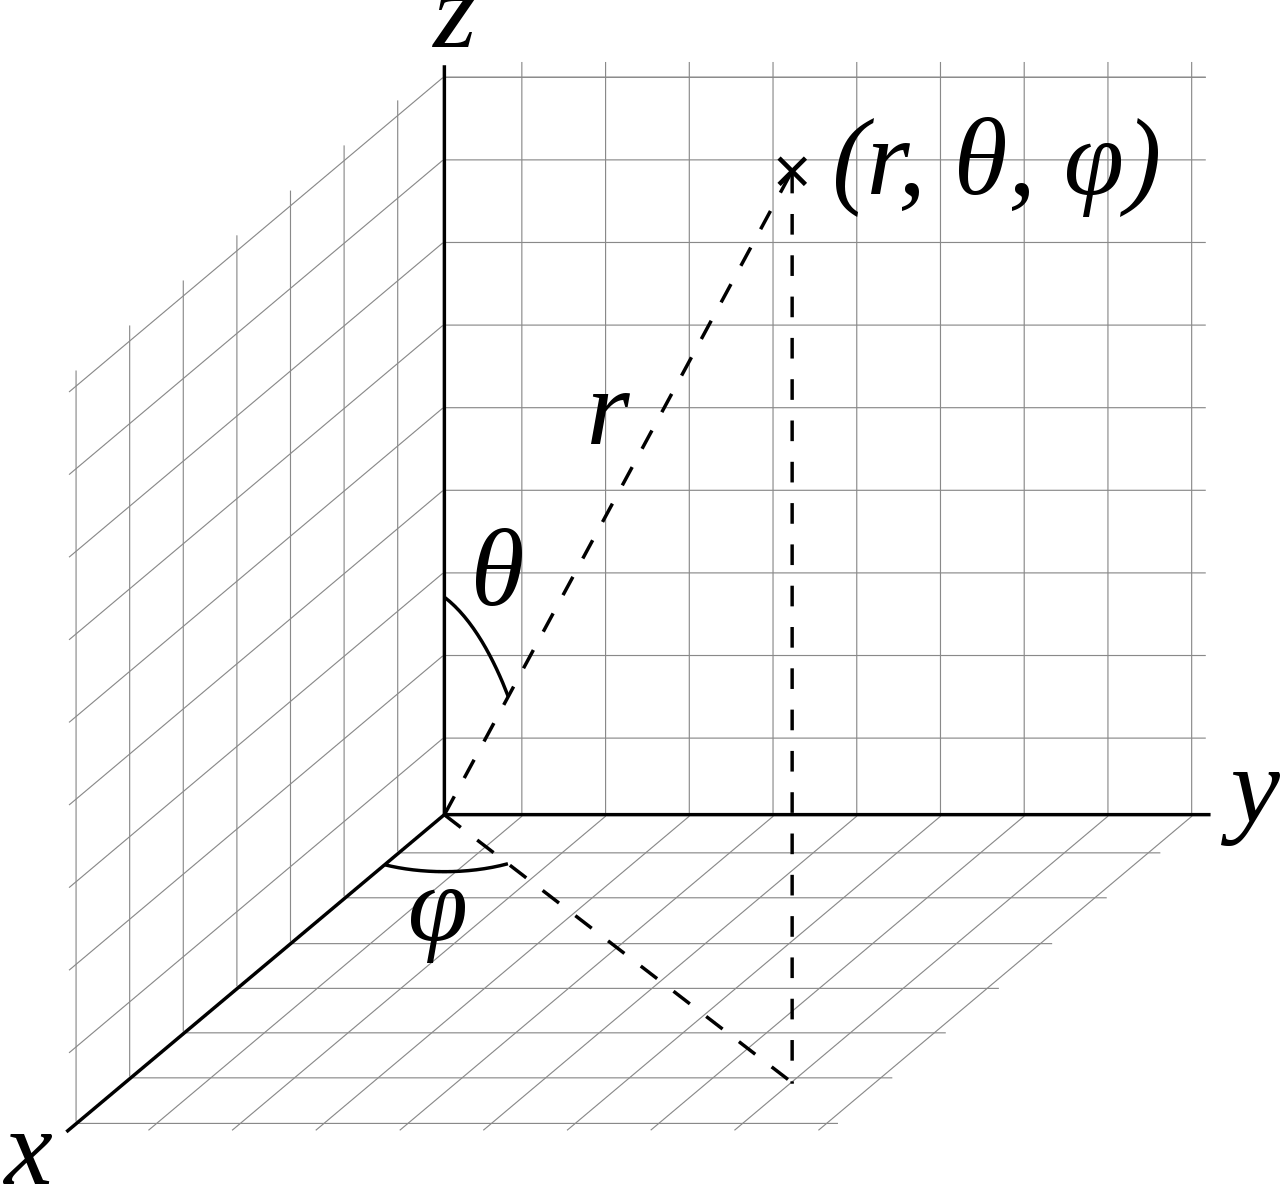
\includegraphics[width=0.75\linewidth]{Spherical-Coordinate-System.png}
\caption{Generic Representation of 3D Spherical Coordinate System.}
\end{center}
\end{figure}
\newline
\newline
Particles are subject to being measured can have any orientation with any value of $\theta$ or $\phi$. Typically these particles that are being described are spin - $1/2$ particles. We will now begin to discuss spin - $1/2$ particles that are present in a magnetic field.
%---------------------------------------------------------------------------
%	Classical Spin - 1/2 Paricles
%---------------------------------------------------------------------------
\section*{Classical Spin - $1/2$ Particles}
Spin - $1/2$ particles can exist in one of two states. The first state can be when these particles are considered to be ``positive" or orientated such that they are parallel to the $+Z$ axis. The other state can be when these particles are ``negative" or orientated such that they are parallel to the $-Z$ axis. Often one can read an academic article where the states of these particles are said to be ``noisy", which essentially means the collection of these particles are almost 50/50 in some being negative and others being positive.

When these particles are present within a magnetic field they have a tendency to ``flip". This flipping phenomenon is when the particles go from being in their positive to negative state or vice versa. For the sake of simplicity we will begin by taking a look at these particles that are present in a constant uniform magnetic field.
%--------------------------------------------------
%	Figure 2
%--------------------------------------------------
\begin{figure}[htbp]
\begin{center}
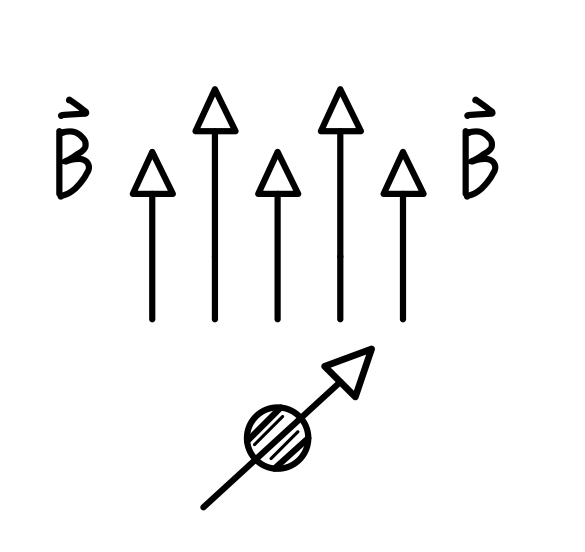
\includegraphics[width=0.75\linewidth]{Dipole-In-Magnetic-Field.PNG}
\caption{Dipole Present in a Magnetic Field.}
\end{center}
\end{figure}
\newline
Figure 2 is an artists rendition of a magnetic dipole that is in presence of a magnetic field. As the dipole is subjected to the magnetic field we should expect it to flip from one orientation to the other, this of course is dependent upon the initial orientation of the dipole. The torque that this dipole experiences can be calculated via
%--------------------------------------------------
%	Equation (1)
%--------------------------------------------------
\begin{equation}
\hat{\tau}=\hat{\mu} \times \hat{B}
\end{equation}
where $\hat{\mu}$ is the dipole moment and $\hat{B}$ is the magnetic field that it is experiencing. Using Isaac Newton's second law we can relate torque to
%--------------------------------------------------
%	Equation (2)
%--------------------------------------------------
\begin{equation}
\frac{d\hat{L}}{dt}=\hat{\tau}
\end{equation}
where $\hat{L}$ is the angular momentum of our particle. It turns out that $\hat{L}$ and $\hat{\mu}$ are proportional via
%--------------------------------------------------
%	Equation (3)
%--------------------------------------------------
\begin{equation}
\hat{L}=\frac{1}{\gamma}\hat{u}
\end{equation}
where $\gamma$ is dependent upon the situation that we are presented with. Finally we can represent the equation of motion for our dipole via
%--------------------------------------------------
%	Equation (4)
%--------------------------------------------------
\begin{equation}
\frac{d\hat{M}}{dt}=\gamma \hspace{2pt} (\hat{M} \times \hat{B})
\end{equation}
where $M=\Sigma \hspace{2pt} \hat{\mu}$. The next task is to solve equation (4) for each direction so that we can have a quantitative description of how our particle interacts with the magnetic field.
%---------------------------------------------------------------------------
%	Solving Equations of Emotion for Dipole
%---------------------------------------------------------------------------
\section*{Solving Equations of Emotion}
Equation (4) describes how we can measure magnetization of these spin - $1/2$ particles. There are three separate equations of emotion for the $x,\hspace{1pt}y,$ and $z$ directions. Those equations are
%--------------------------------------------------
%	Equation (5,6,7)
%--------------------------------------------------
\begin{equation}
\frac{dM_{x}}{dt}=\gamma(\hat{M}\times\hat{B})_{x}-\frac{M_{x}}{T_{2}},
\end{equation}
\begin{equation}
\frac{dM_{y}}{dt}=\gamma(\hat{M}\times\hat{B})_{y}-\frac{M_{y}}{T_{2}},
\end{equation}
\begin{equation}
\frac{dM_{z}}{dt}=\frac{M_{0}-M_{z}}{T_{1}}
\end{equation}
where $T_1$ and $T_2$ are parameters for a given situation. Equations (5) and (6) simplify significantly with the only magnetic field that is non zero is the $\hat{B}_z$. After separating variables and solving the differential equations the solutions to equations (5) and (6) are
%--------------------------------------------------
%	Equation (8)
%--------------------------------------------------
\begin{equation}
M_{x}=A\sin{(\gamma B_{z}t)}-B\cos{(\gamma B_{z}t)}
\end{equation}
%--------------------------------------------------
%	Equation (9)
%--------------------------------------------------
and
\begin{equation}
M_{y}=A\cos{(\gamma B_{z}t)}+B\sin{(\gamma B_{z}t)}.
\end{equation}
Equations (8) and (9) describe the rate at which the particles rotate in the $x-y$ plane classically. The solution to equation (7)
%--------------------------------------------------
%	Equation (10)
%--------------------------------------------------
\begin{equation}
M_{z}=M_{zi}e^{(-\frac{t}{T_1})}+M_{0}(1-e^{(-\frac{t}{T_1})})
\end{equation}
where equation (10) describes the rate of change that the spin - $1/2$ particle rotates from spin up ($+z$ orientation) to spin down ($-z$ orientation) or vice versa. Now that equations (5), (6), and (7) have been solved we can move on to examining these spin - $1/2$ in a different light.
%---------------------------------------------------------------------------
%	Quantum Spin - 1/2 Systems
%---------------------------------------------------------------------------
\section*{Quantum Spin - $1/2$ Systems}
There are ways that we can describe these spin - $1/2$ systems with the language of Quantum Mechanics. Conversely Quantum Mechanics can be described in the language of linear algebra, specifically in this case with bras and kets. These spin - $1/2$ systems can be described with the ket 
%--------------------------------------------------
%	Equation (11)
%--------------------------------------------------
\begin{equation}
\ket{\psi}=a_{+}\ket{+\hat{z}}+a_{-}\ket{-\hat{z}}
\end{equation}
where $a_{+}$ and $a_{-}$ are normalization constants. When we subject these particles to a measurement in either the $x, \hspace{1pt} y$, or $z$ direction we have the possibility of getting one of two outcomes. The two possible outcomes from this measurement are $+\hbar/2$ and $-\hbar/2$ and this scheme can be seen in Figure 3 below. \\
%--------------------------------------------------
%	Figure 3
%--------------------------------------------------
\begin{figure}[htpb]
\begin{center}
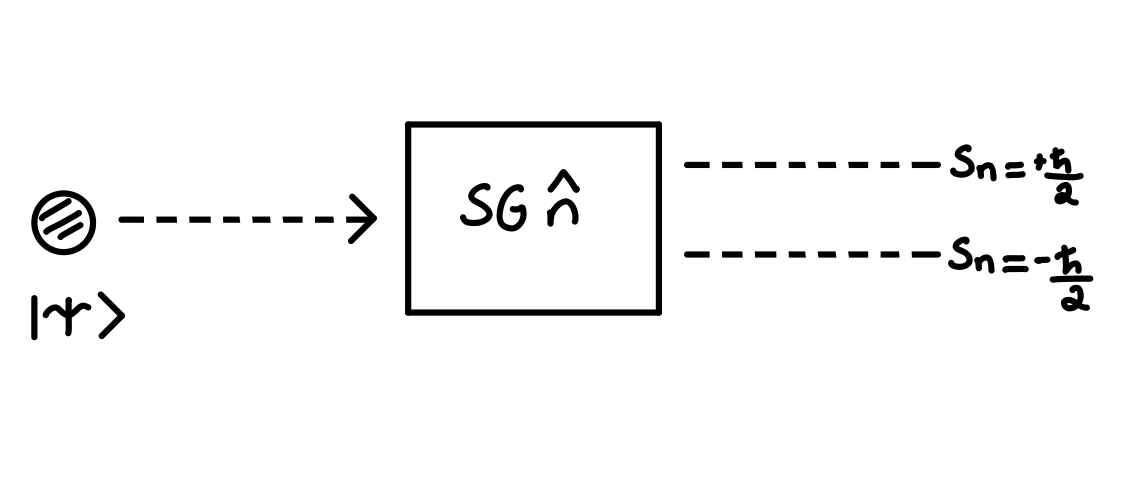
\includegraphics[width=0.90\linewidth]{SG-Measurement.PNG}
\caption{Artistic Rendition of SG Measurement.}
\end{center}
\end{figure}
\newline
Figure 3 encompasses a generic state $\hat{n}$ which can either be the $x, \hspace{1pt} y$, or $z$ direction. These states can represent the $x, \hspace{1pt} y$, or $z$ direction by knowing $\theta$ and $\phi$ for whatever particle we are interested in measuring. These states can be calculated by
%--------------------------------------------------
%	Equations (12)
%--------------------------------------------------
\begin{equation}
\ket{+\hat{n}}=\cos{(\theta/2)}\ket{+\hat{z}}+e^{i\phi}\sin{(\theta/2)}\ket{-\hat{z}}
\end{equation}
and
%--------------------------------------------------
%	Equations (13)
%--------------------------------------------------
\begin{equation}
\ket{-\hat{n}}=\sin{(\theta/2)}\ket{+\hat{z}}-e^{i\phi}\cos{(\theta/2)}\ket{-\hat{z}}.
\end{equation}
Once these states are known we can also calculate the probabilities of getting $+\hbar/2$ and $-\hbar/2$ by
%--------------------------------------------------
%	Equation (14)
%--------------------------------------------------
\begin{equation}
\text{Prob}=|\bra{\pm\hat{n}}\ket{\psi}|^2
\end{equation}
where the probabilities of getting $+\hbar/2$ and $-\hbar/2$ must add up to be 1.

Using linear algebra we can also right certain ket vectors in terms of $\pm\ket{\hat{n}}$. Take for instance the ket vector
%--------------------------------------------------
%	Equation (15)
%--------------------------------------------------
\begin{equation}
\ket{\psi}=\cos{(\omega t)}\hat{x}+\sin{(\omega t)}\hat{y}.
\end{equation}
Equation (15) exists in the x-y plane and thus $\theta=\pi/2$ and $\phi=\omega t$. Utilizing equations (12) and (13) equation (15) can be written as
%--------------------------------------------------
%	Equations (16,17)
%--------------------------------------------------
\begin{equation}
\ket{+\psi}=\frac{1}{\sqrt{2}}\ket{+\hat{z}}+\frac{1}{\sqrt{2}}e^{i\omega t}\ket{-\hat{z}}
\end{equation}
and
\begin{equation}
\ket{-\psi}=\frac{1}{\sqrt{2}}\ket{+\hat{z}}-\frac{1}{\sqrt{2}}e^{i\omega t}\ket{-\hat{z}}.
\end{equation}
Now that we know equation (16) and (17) we can calculate the probability of measuring both $\hbar/2$ and $-\hbar/2$ with certainty in whatever direction we choose by using equation (14). First we measure the $+\hat{z}$ direction and get
%--------------------------------------------------
%	Equations (18,19)
%--------------------------------------------------
\begin{equation}
|\bra{+\hat{z}}\ket{+\psi}|^2=1/2
\end{equation}
and conversely the $-\hat{z}$ direction we get 
\begin{equation}
|\bra{-\hat{z}}\ket{+\psi}|^2=1/2.
\end{equation}
Calculating these probabilities with $+\psi$ and $-\psi$ will result the same probabilities and it is thus redundant to show the probabilities with $-\psi$ if we show the $+\psi$ probabilities. We can now work on calculating the probabilities of getting $\hbar/2$ and $-\hbar/2$ with certainty for the $\hat{x}$ and $\hat{y}$ directions. First we will examine the $+\hat{x}$ and get
%--------------------------------------------------
%	Equations (20,21)
%--------------------------------------------------
\begin{equation}
|\bra{+\hat{x}}\ket{+\psi}|^2=\frac{1}{2}(1+\cos{(\omega t)})
\end{equation}
where the $-\hat{x}$ is
\begin{equation}
|\bra{-\hat{x}}\ket{+\psi}|^2=\frac{1}{2}(1-\cos{(\omega t)})
\end{equation}
where the probabilities of measuring $\hbar/2$ and $-\hbar/2$ with certainty depend upon the angular frequency $\omega$ and the time $t$. The $y$ directions thus yield
%--------------------------------------------------
%	Equations (22,23)
%--------------------------------------------------
\begin{equation}
|\bra{+\hat{y}}\ket{+\psi}|^2=\frac{1}{2}(1+\sin{(\omega t)})
\end{equation}
where the $-\hat{y}$ gives us
\begin{equation}
|\bra{-\hat{y}}\ket{+\psi}|^2=\frac{1}{2}(1-\sin{(\omega t)})\end{equation}
where the probabilities from (22) and (23) are bound by the angular frequency $\omega$ and the time $t$ as well.
%---------------------------------------------------------------------------
%	Spin - 1/2 in |0> and |1>
%---------------------------------------------------------------------------
\section*{Spin - 1/2 Particles in $\ket{0}$ and $\ket{1}$ Notation}
It is not usual to use $+\ket{z}$ and $-\ket{z}$ for notation in describing the states of spin - 1/2 particles. It is convention to use $\ket{0}$ for $+\ket{z}$ and $\ket{1}$ for $-\ket{z}$ when describing spin - 1/2 particles. Using the new kets to describe a particle we can write equations (12) and (13) as
%--------------------------------------------------
%	Equations (24,25)
%--------------------------------------------------
\begin{equation}
\ket{+\hat{n}}=\cos{(\theta/2)}\ket{0}+e^{i\phi}\sin{(\theta/2)}\ket{1}
\end{equation}
and
\begin{equation}
\ket{-\hat{n}}=\sin{(\theta/2)}\ket{0}-e^{i\phi}\cos{(\theta/2)}\ket{1}.
\end{equation}
We can thus express $+\ket{\hat{z}}$ and $-\ket{\hat{z}}$ by using the equations (24) and (25) with the values for $\theta=0$ and $\phi=0$. The $+z$ direction is thus
%--------------------------------------------------
%	Equations (26,27)
%--------------------------------------------------
\begin{equation}
\ket{+\hat{z}}=\ket{0}
\end{equation}
and
\begin{equation}
\ket{-\hat{z}}=-\ket{1}.
\end{equation}
We can do the same for the x and y directions. The x direction has $\theta = \pi/2$ and $\phi=0$ for the angles and the equation for x is
%--------------------------------------------------
%	Equations (28,29)
%--------------------------------------------------
\begin{equation}
\ket{+\hat{x}}=\frac{1}{\sqrt{2}}\ket{0}+\frac{1}{\sqrt{2}}\ket{1}
\end{equation}
and the -x is
\begin{equation}
\ket{-\hat{x}}=\frac{1}{\sqrt{2}}\ket{0}-\frac{1}{\sqrt{2}}\ket{1}.
\end{equation}
The y-direction has $\theta=\pi/2$ and $\phi=\pi/2$ and the equation for y is
%--------------------------------------------------
%	Equations (30,31)
%--------------------------------------------------
\begin{equation}
\ket{+\hat{y}}=\frac{1}{\sqrt{2}}\ket{0}+\frac{i}{\sqrt{2}}\ket{1}
\end{equation}
and the -y is
\begin{equation}
\ket{-\hat{y}}=\frac{1}{\sqrt{2}}\ket{0}-\frac{i}{\sqrt{2}}\ket{1}.
\end{equation}
Now that we described x,y, and z with $\ket{0}$ and $\ket{1}$ we can begin to examine states written in this notation. Take for instance these states
%--------------------------------------------------
%	Equations (32,33,34,35)
%--------------------------------------------------
\begin{equation}
\Big\{ \frac{1}{\sqrt{2}}\big(\ket{0} + \ket{1}\big), \frac{1}{\sqrt{2}}\big(\ket{0}+i\ket{1}\big)\Big\},
\end{equation}
\begin{equation}
\Big\{ \frac{1}{\sqrt{2}}\big(\ket{0} + \ket{1}\big), \frac{1}{\sqrt{2}}\big(\ket{0}-\ket{1}\big)\Big\},
\end{equation}
\begin{equation}
\Big\{ \frac{1}{5}\big(3\ket{0}+4i\ket{1}\big), \frac{1}{5}\big(4\ket{0}-3i\ket{1}\big)\Big\},
\end{equation}
\begin{equation}
\Big\{\frac{1}{5}\big(3\ket{0}+4i\ket{1}\big), \frac{1}{5}\big(4\ket{0}+3i\ket{1}\big)\Big\}.
\end{equation}
We are tasked if determining if the states in equations (32) - (35) are measurement bases. Mathematically, if multiplying the states together in equations (32) - (35) are 0, that means the corresponding states are orthogonal and thus are measurement bases. It turns out that equations (33) and (34) are orthogonal to each other and are thus measurement bases. Equations (32) and (35) are not orthogonal to one another and are thus not measurement bases.

We move on now from examining orthogonality amongst states to discuss qualitative Stern Gerlach measurements and what we can learn and what we should expect in repeated measurements. Take for instance the scenario in the Figure 4 below.
%--------------------------------------------------
%	Figure 4
%--------------------------------------------------
\begin{figure}[htpb]
\begin{center}
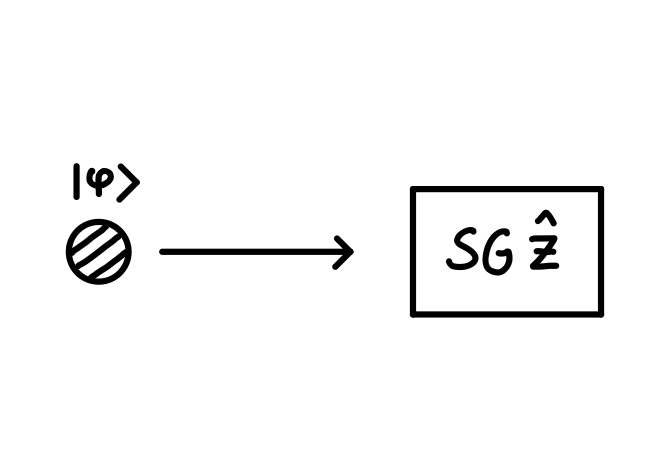
\includegraphics[width=0.70\linewidth]{SG-Measurement-Z-One-Time.PNG}
\caption{Stern Gerlach Measurement Along the Z Direction.}
\end{center}
\end{figure}
The particle that is subject to a measurement in the $\hat{z}$ direction is
%--------------------------------------------------
%	Equation (36)
%--------------------------------------------------
\begin{equation}
\ket{\psi}=\cos{(\theta/2)}\ket{0}+\sin{(\theta/2)}\ket{1}
\end{equation}
where $\phi=0$ in this instance. In this scenario we are tasked with learning about the value of $\theta$ in equation (36). If we measure the $-\hat{z}$ of this particle we get the following result
%--------------------------------------------------
%	Equation (37)
%--------------------------------------------------
\begin{equation}
\bra{-\hat{z}}\ket{\psi}=-\sin{(\theta/2)}
\end{equation}
and from this we know that $\theta \neq 0$ because if $\theta$ were zero the probability of measuring $-\hbar/2$ with certainty would be zero. In essence, conversely if we measure 
%--------------------------------------------------
%	Equation (38)
%--------------------------------------------------
\begin{equation}
\bra{\hat{z}}\ket{\psi}=\cos{(\theta/2)}
\end{equation}
and we would learn from this measurement that $\theta \neq \pi$ because this would again yield a probability of $0$ for measuring $\hbar/2$ with certainty and that is not possible. We can perform the same measurement in the x-direction and try to learn $\theta$ that way for equation (36). First we examine the scenario below in terms of a cartoon.
%--------------------------------------------------
%	Figure 5
%--------------------------------------------------
\begin{figure}[htpb]
\begin{center}
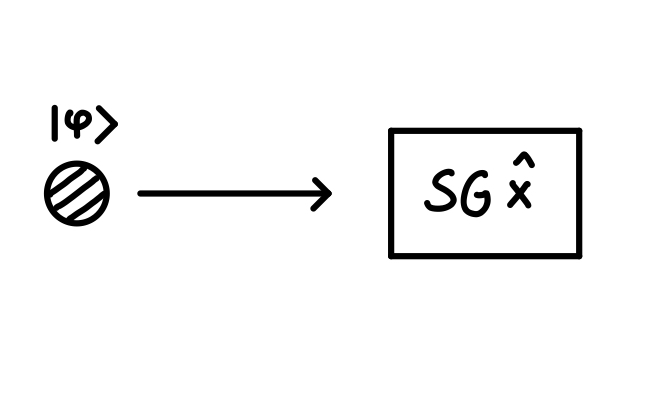
\includegraphics[width=0.70\linewidth]{SG-Measurement-X-One-Time.PNG}
\caption{Stern Gerlach Measurement Along the X Direction.}
\end{center}
\end{figure}
\newline
We now repeat the measurement for $\psi$ in the x-direction to try and determine what the value of $\theta$ can be. Measuring the $-\hat{x}$ direction we get
%--------------------------------------------------
%	Equation (39)
%--------------------------------------------------
\begin{equation}
\bra{-\hat{x}}\ket{\psi}=\frac{1}{2}(1-\sin{(\theta)})
\end{equation}
and from this we learn that $\theta \neq \pi/2$ because this would again yield a zero possibility for measuring $-\hbar/2$ with certainty. We do the same thing and now measure the x direction and get
%--------------------------------------------------
%	Equation (40)
%--------------------------------------------------
\begin{equation}
\bra{+\hat{x}}\ket{\psi}=\frac{1}{2}(1+\sin{(\theta)})
\end{equation}
where this result tells us that $\theta \neq 3\pi/2$ due to us getting a zero probability for measuring $\hbar/2$ with certainty at this given angle. From the results of (37 - 40) we have learned more or less what values of $\theta$ there cannot be. These results have yielded values that show we cannot have $\theta$ at specific angles rather than what the actual value of $\theta$ there is in equation (36). We now move on to making more qualitative observations about similar scenarios that are seen in Figure 4 and Figure 5.

We now observe the scenario of a repeated measurement of $\psi$ as seen in Figure 6 below.
%--------------------------------------------------
%	Figure 6
%--------------------------------------------------
\begin{figure}[htpb]
\begin{center}
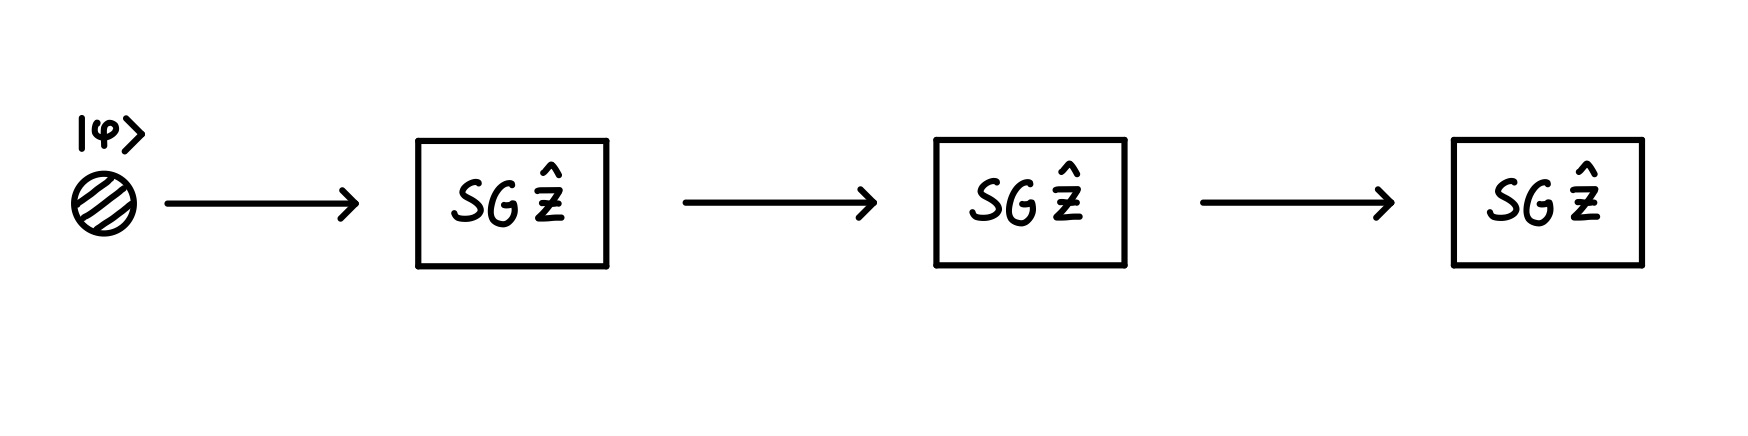
\includegraphics[width=0.90\linewidth]{SG-Measurement-Z-Three-Times.PNG}
\caption{Repeated Stern Gerlach Z Measurement.}
\end{center}
\end{figure}
\newline
Figure 6 depicts a state $\ket{\psi}$ being measured multiple times in the z direction and the question that arises is if we will learn any additional information about $\ket{\psi}$ after the first z measurement. The answer is we will not learn any new information about $\ket{\psi}$ after the first measurement because the outcomes that come out are repeated over and over after the first z measurement. Instead we now look at a different scenario depicted in Figure 7.
%--------------------------------------------------
%	Figure 7
%--------------------------------------------------
\begin{figure}[htpb]
\begin{center}
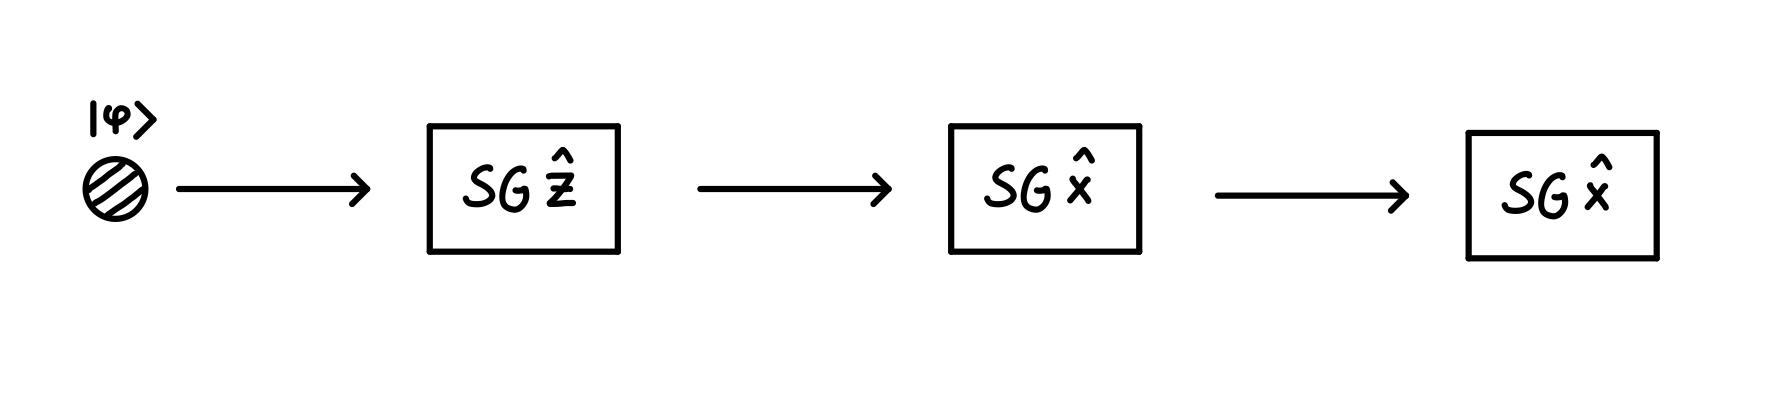
\includegraphics[width=0.90\linewidth]{SG-Measurement-Mixed.PNG}
\caption{Repeated Mixed Measurement.}
\end{center}
\end{figure}
\newline
First the state $\ket{\psi}$ is measured in the z-direction and then it is measured in the x-direction twice. In this scenario we are tasked if measuring in the x-direction is affected by measuring in the z-direction first. The short answer is no because we can get $\hbar/2$ and $-\hbar/2$ as an answer for the x measurements and that is no different of an outcome from the measurement that occurs in the z-direction. We now move onto more examination of these states.

Consider the following states
%--------------------------------------------------
%	Equations (41 - 43)
%--------------------------------------------------
\begin{equation}
\ket{\psi}=\frac{1}{5}\big(3\ket{0} + 4\ket{1}\big),
\end{equation}
\begin{equation}
\ket{\psi}=\frac{1}{5}\big(3\ket{0} + 4i\ket{1}\big),
\end{equation}
\begin{equation}
\ket{\psi}=\frac{1}{13}\big(12\ket{0} - 5i\ket{1}\big)
\end{equation}
where the task with these states is to determine at what angle $\theta$ and $\phi$ our Stern Gerlach apparatus must be oriented such that we measure $\hbar/2$ with certainty. It turns out for our first state, equation (41), the angles are $\theta=106\degree$ and $\phi=0\degree$ will give us the corresponding state. For equation (42) the angles are $\theta=106\degree$ and $\phi=90\degree$ and equation (43) has angles of $\theta=45\degree$ and $\phi=270\degree$ that will produce $\hbar/2$ as a measurement with certainty. The last task with equations (41), (42), and (43) is to measure the probabilities of measuring $\hbar/2$ and $-\hbar/2$ with certainty for the x and z-directions.

First we begin by examining the probability of measuring $\hbar/2$ with certainty for the x-direction. For equations (41), (42), and (43) the probabilities for measuring $\hbar/2$ with certainty for x-direction are
%--------------------------------------------------
%	Equation (44)
%--------------------------------------------------
\begin{equation}
|\bra{+\hat{x}}\ket{\psi}|^2=\frac{49}{50},
\end{equation}
\begin{equation}
|\bra{+\hat{x}}\ket{\psi}|^2=\frac{1}{2},
\end{equation}
and
\begin{equation}
|\bra{+\hat{x}}\ket{\psi}|^2=\frac{1}{2}.
\end{equation}
The probabilities of measuring $-\hbar/2$ with certainty in the negative x-direction for equations (41), (42), and (43) are
\begin{equation}
|\bra{-\hat{x}}\ket{\psi}|^2=\frac{1}{50},
\end{equation}
\begin{equation}
|\bra{-\hat{x}}\ket{\psi}|^2=\frac{1}{2},
\end{equation}
and
\begin{equation}
|\bra{-\hat{x}}\ket{\psi}|^2=\frac{1}{2}.
\end{equation}
We can do the same thing for the z-direction as we did with the x-direction. Starting with the z-direction the probabilities for measuring $\hbar/2$ with certainty for equations (41), (42), and (43) are
\begin{equation}
|\bra{+\hat{z}}\ket{\psi}|^2=\frac{9}{25},
\end{equation}
\begin{equation}
|\bra{+\hat{z}}\ket{\psi}|^2=\frac{9}{25},
\end{equation}
and
\begin{equation}
|\bra{+\hat{z}}\ket{\psi}|^2=\frac{144}{169}.
\end{equation}
The probabilities of measuring $-\hbar/2$ with certainty for the negative z-direction for equations (41), (42), and (43) are
\begin{equation}
|\bra{-\hat{z}}\ket{\psi}|^2=\frac{16}{25},
\end{equation}
\begin{equation}
|\bra{-\hat{z}}\ket{\psi}|^2=\frac{16}{25},
\end{equation}
and
\begin{equation}
|\bra{-\hat{z}}\ket{\psi}|^2=\frac{25}{169}.
\end{equation}
This concludes our examination of bra and ket vectors in terms of $\ket{0}$ and $\ket{1}$.
%---------------------------------------------------------------------------
%	Entangled and Product States
%---------------------------------------------------------------------------
\section*{Entangled and Product States}
We continue our investigation into spin - 1/2 particles by examining entangled and product states. In short, entangled states and product states are states that involve multiple states. Product states are two states of which that can be separated into two separate individual states. Entangled states are states that involve two states that cannot be separated such that each individual state can be recognized. Before we start investigating product and entangled states we will examine one more individual state.

We continue our investigation of spin - 1/2 particles. Consider a collection of spin - 1/2 particles that are all originally in the state
%--------------------------------------------------
%	Equation (56)
%--------------------------------------------------
\begin{equation}
\ket{\psi}=\cos{(\alpha/2)}\ket{0}+\sin{(\alpha/2)}\ket{1}
\end{equation}
where there will be of collection of N total measurements. Each measurement yields the possibility of either measuring $\hbar/2$ and $-\hbar/2$ with certainty. We are tasked with determining the $\alpha$ angle in equation (56) by taking measurements in the x, y, and z-directions. By first measuring the z-direction with $\ket{\psi}$ we get the following probability of measuring $\hbar/2$ with certainty
%--------------------------------------------------
%	Equation (57)
%--------------------------------------------------
\begin{equation}
|\bra{+\hat{z}}\ket{\psi}|^2=\cos^2{(\alpha/2)}=\frac{n_+}{N}.
\end{equation}
The, ``$n_+$" that is seen in equation (57) is the amount of times $\hbar/2$ would be measured in an experiment with N number of total measurements. Conversely the probability of measuring $-\hbar/2$ with certainty in the z-direction is
%--------------------------------------------------
%	Equation (58)
%--------------------------------------------------
\begin{equation}
|\bra{-\hat{z}}\ket{\psi}|^2=\sin^2{(\alpha/2)}=\frac{n_-}{N}.
\end{equation}
Similar to equation (57), ``$n_-$" is the amount of times $-\hbar/2$ would be measured in an experiment with N number of total measurements. By solving equations (57) and (58) for $\alpha$ we can determine $\alpha$ and thus know how $\ket{\psi}$ is oriented. We can also do the same with the x-direction as we did with the z-direction.

By first calculating the probability of measuring $\hbar/2$ with certainty in the x-direction we get
%--------------------------------------------------
%	Equation (59)
%--------------------------------------------------
\begin{equation}
|\bra{+\hat{x}}\ket{\psi}|^2=\frac{1}{2}\big(1+\sin{(\alpha)}\big)=\frac{n_+}{N}.
\end{equation}
We can see that equation (57) and (59) are different and that is due to measuring in different directions. Calculating the probability of measuring $-\hbar/2$ in the x-direction we get
%--------------------------------------------------
%	Equation (60)
%--------------------------------------------------
\begin{equation}
|\bra{-\hat{x}}\ket{\psi}|^2=\frac{1}{2}\big(1-\sin{(\alpha)}\big)=\frac{n_-}{N}.
\end{equation}
The differences between (57), (59), (58), and (60) are apparent and the question arises as to which equations best approximate $\alpha$ with the smallest amount of deviation. This question can be answered by calculating what is called the Fisher information and that will be discussed in more detail later on in this paper. 

By measuring in the y-direction we got a probability of 1/2 for $\hbar/2$ and for $-\hbar/2$ that did not depend on the angle $\alpha$. Because of this, we were not able to learn anything about $\alpha$. Therefore equations (57) through (60) are the only appropriate ways measuring $\alpha$. We will now begin our investigation of product and entangled states.

Take for instance the state
%--------------------------------------------------
%	Equation (61)
%--------------------------------------------------
\begin{equation}
\ket{\psi}=\frac{1}{2}\big(\ket{0}\ket{0}+\ket{0}\ket{1}-\ket{1}\ket{0}-\ket{1}\ket{1}\big)
\end{equation}
which for instance is an example of a product state. Equation (61) can be written as a combination of states such that
%--------------------------------------------------
%	Equation (62)
%--------------------------------------------------
\begin{equation}
\ket{\psi}=\ket{\psi_A}\ket{\psi_B}.
\end{equation}
Precisely $\ket{\psi_A}$ can be written as
%--------------------------------------------------
%	Equation (63)
%--------------------------------------------------
\begin{equation}
\ket{\psi_A}=\frac{-1}{\sqrt{2}}\ket{0}+\frac{1}{\sqrt{2}}\ket{1}
\end{equation}
and $\ket{\psi_B}$ can be written as
%--------------------------------------------------
%	Equation (64)
%--------------------------------------------------
\begin{equation}
\ket{\psi_B}=\frac{-1}{\sqrt{2}}\ket{0}-\frac{1}{\sqrt{2}}\ket{1}.
\end{equation}
When equation (63) and (64) are multiplied together equation (61) is produced. Similar to single states, product states can have probabilities calculated. Table 1 depicts the probability getting a combination of measurements for this entangled state with the positive state being $\ket{0}$ and the negative state being $\ket{1}$.
%--------------------------------------------------
%	Table 1
%--------------------------------------------------
\begin{table}[h!]
\begin{center}
\begin{tabular}{ |c|c|c|c| }
\hline SG $\hat{z}$ A& SG $\hat{z}$ B& State& Probability \\ 
\hline +& +& $\ket{0}$,$\ket{0}$& 1/4 \\  
\hline +& -& $\ket{0}$,$\ket{1}$& 1/4 \\
\hline -& +& $\ket{1}$,$\ket{0}$& 1/4 \\
\hline -& -& $\ket{1}$,$\ket{1}$& 1/4 \\
\hline    
\end{tabular}
\caption{Probabilities of States for A in SG $\hat{z}$ and B in SG $\hat{z}$.}
\end{center}
\end{table} \\
We can also examine probabilities with different directions. For instance we can measure the probabilities of SG $\hat{x}$ for A and SG $\hat{z}$ for B. The positive state in the $\hat{x}$ is $\frac{\ket{0}+\ket{1}}{\sqrt{2}}$ and the negative state is $\frac{\ket{0}-\ket{1}}{\sqrt{2}}$. The results of measuring the probabilities of these states in their respective directions can be seen in Table 2.
%--------------------------------------------------
%	Table 2
%--------------------------------------------------
\begin{table}[h!]
\begin{center}
\begin{tabular}{ |c|c|c|c| }
\hline SG $\hat{x}$ A& SG $\hat{z}$ B& State& Probability \\ 
\hline +& +& $\frac{\ket{0}+\ket{1}}{\sqrt{2}}$,$\ket{0}$& 0 \\  
\hline +& -& $\frac{\ket{0}+\ket{1}}{\sqrt{2}}$,$\ket{1}$& 0 \\
\hline -& +& $\frac{\ket{0}-\ket{1}}{\sqrt{2}}$,$\ket{0}$& 1/2 \\
\hline -& -& $\frac{\ket{0}-\ket{1}}{\sqrt{2}}$,$\ket{1}$& 1/2 \\
\hline    
\end{tabular}
\caption{Probabilities of States for A in SG $\hat{x}$ and B in SG $\hat{z}$.}
\end{center}
\end{table}
\newpage
We can see here in Table 2 that there are only two states that have a non zero probability. This only occurs when State A is negative. The last scenario that was observed with this state occurs when we measure SG $\hat{x}$ for A and SG $\hat{x}$ for B. The probabilities of these measurements can be seen in Table 3.
%--------------------------------------------------
%	Table 3
%--------------------------------------------------
\begin{table}[h!]
\begin{center}
\begin{tabular}{ |c|c|c|c| }
\hline SG $\hat{x}$ A& SG $\hat{x}$ B& State& Probability \\ 
\hline +& +& $\frac{\ket{0}+\ket{1}}{\sqrt{2}}$,$\frac{\ket{0}+\ket{1}}{\sqrt{2}}$& 0 \\  
\hline +& -& $\frac{\ket{0}+\ket{1}}{\sqrt{2}}$,$\frac{\ket{0}-\ket{1}}{\sqrt{2}}$& 0 \\
\hline -& +& $\frac{\ket{0}-\ket{1}}{\sqrt{2}}$,$\frac{\ket{0}+\ket{1}}{\sqrt{2}}$& 1 \\
\hline -& -& $\frac{\ket{0}-\ket{1}}{\sqrt{2}}$,$\frac{\ket{0}-\ket{1}}{\sqrt{2}}$& 0 \\
\hline    
\end{tabular}
\caption{Probabilities of States for A in SG $\hat{x}$ and B in SG $\hat{x}$.}
\end{center}
\end{table}
\\
The results from Table 3 show that there is one pair of measurements that yield an outcome with certainty. All the other measurements have a zero probability except for the positive A state and the negative B state. We now continue a similar investigation with an entangled state rather than a product state.

Consider the following entangled state
%--------------------------------------------------
%	Equation (65)
%--------------------------------------------------
\begin{equation}
\ket{\psi}=\frac{1}{2}\big(\ket{0}\ket{0}+\ket{0}\ket{1}+\ket{1}\ket{0}-\ket{1}\ket{1}\big).
\end{equation}
Equation (65) cannot be split up into two separate states and therefore that is what makes this state entangled. We can again compute the probabilities with this state that is depicted in equation (65). The first measurement we will make with this state is the SG $\hat{z}$ for A and SG $\hat{z}$ for B. That states that are being measured with equation (65) are the same as with equation (61). The results of measuring the probabilities of this state can be seen in Table 4.
%--------------------------------------------------
%	Table 4
%--------------------------------------------------
\begin{table}[h!]
\begin{center}
\begin{tabular}{ |c|c|c|c| }
\hline SG $\hat{z}$ A& SG $\hat{z}$ B& State& Probability \\ 
\hline +& +& $\ket{0}$,$\ket{0}$& 1/4 \\  
\hline +& -& $\ket{0}$,$\ket{1}$& 1/4 \\
\hline -& +& $\ket{1}$,$\ket{0}$& 1/4 \\
\hline -& -& $\ket{1}$,$\ket{1}$& 1/4 \\
\hline    
\end{tabular}
\caption{Probabilities of States for A in SG $\hat{z}$ and B in SG $\hat{z}$.}
\end{center}
\end{table} \\
The probabilities of these measurements are again the same as with the results seen in Table 1. Continuing with the trend, we are going to now measure the SG $\hat{x}$ for A and $\hat{z}$ for B with equation (65). The results of measuring these probabilities can be seen in Table 5.
%--------------------------------------------------
%	Table 5
%--------------------------------------------------
\begin{table}[h!]
\begin{center}
\begin{tabular}{ |c|c|c|c| }
\hline SG $\hat{x}$ A& SG $\hat{z}$ B& State& Probability \\ 
\hline +& +& $\frac{\ket{0}+\ket{1}}{\sqrt{2}}$,$\ket{0}$& 1/2 \\  
\hline +& -& $\frac{\ket{0}+\ket{1}}{\sqrt{2}}$,$\ket{1}$& 0 \\
\hline -& +& $\frac{\ket{0}-\ket{1}}{\sqrt{2}}$,$\ket{0}$& 0 \\
\hline -& -& $\frac{\ket{0}-\ket{1}}{\sqrt{2}}$,$\ket{1}$& 1/2 \\
\hline    
\end{tabular}
\caption{Probabilities of States for A in SG $\hat{x}$ and B in SG $\hat{z}$.}
\end{center}
\end{table} \\
The last states to be examined with equation (65) is SG $\hat{x}$ for A and SG $\hat{x}$ for B and these results can be seen in Table 6.
%--------------------------------------------------
%	Table 6
%--------------------------------------------------
\begin{table}[h!]
\begin{center}
\begin{tabular}{ |c|c|c|c| }
\hline SG $\hat{x}$ A& SG $\hat{x}$ B& State& Probability \\ 
\hline +& +& $\frac{\ket{0}+\ket{1}}{\sqrt{2}}$,$\frac{\ket{0}+\ket{1}}{\sqrt{2}}$& 1/4 \\  
\hline +& -& $\frac{\ket{0}+\ket{1}}{\sqrt{2}}$,$\frac{\ket{0}-\ket{1}}{\sqrt{2}}$& 1/4 \\
\hline -& +& $\frac{\ket{0}-\ket{1}}{\sqrt{2}}$,$\frac{\ket{0}+\ket{1}}{\sqrt{2}}$& 1/4 \\
\hline -& -& $\frac{\ket{0}-\ket{1}}{\sqrt{2}}$,$\frac{\ket{0}-\ket{1}}{\sqrt{2}}$& 1/4 \\
\hline    
\end{tabular}
\caption{Probabilities of States for A in SG $\hat{x}$ and B in SG $\hat{x}$.}
\end{center}
\end{table}
\\
The biggest difference between the results in Table 3 and the results in Table 6 are that there are no measurements with 100\% probability. Instead the measurements in Table 6 have equal probability of being measured. This concludes our investigation of product and entangled states.
%---------------------------------------------------------------------------
%	Measurement Operators
%---------------------------------------------------------------------------
\section*{Measurement Operators}
The next topic of discussion are measurement operators. Measurement operators can be used to determine how a state is affected when it enters a certain physical scenario. These physical scenarios can be a spin - 1/2 particles that enter a magnetic field. When these particles enter magnetic fields they will be reoriented according to their initial orientation. We can use measurement operators to determine such outcomes. Before we start investigating measurement operators we will examine a state and how to determine how it is oriented.

Consider a collection of N number of particles in the original state
%--------------------------------------------------
%	Equation (66)
%--------------------------------------------------
\begin{equation}
\ket{\psi}=\frac{1}{\sqrt{2}}+e^{i\phi}\frac{1}{\sqrt{2}}\ket{1}.
\end{equation}
The first thing that can be examined by the state in equation (66) is that the state is oriented in the x-y plane. This is because $\theta=\pi/2$ and the only unknown angle is $\phi$. We are tasked with trying to figure out $\phi$ by measuring in each direction. Our first observation is that we cannot learn anything about $\phi$ by measuring in the $\hat{z}$ direction. This is because when we measure in the $\hat{z}$ direction we get a probability of 1/2 for measuring both $\hbar/2$ and $-\hbar/2$ with certainty that does not depend upon $\phi$.

Measuring in the $\hat{x}$ direction can however yield information for how to determine $\phi$. When we measure the probability of obtaining $\hbar/2$ with certainty in the $+\hat{x}$ direction we obtain
%--------------------------------------------------
%	Equation (67)
%--------------------------------------------------
\begin{equation}
|\bra{+\hat{x}}\ket{\psi}|^2=\frac{1}{2}\big(1+\cos{(\phi)}\big)=\frac{n_+}{N}.
\end{equation}
In equation (67) the $n_+$ value is how many times $\hbar/2$ would be counted in an experiment that was repeated N number of times. The same procedure can be done with the $-\hat{x}$ direction. The probability of measuring $-\hbar/2$ with certainty is thus
%--------------------------------------------------
%	Equation (68)
%--------------------------------------------------
\begin{equation}
|\bra{-\hat{x}}\ket{\psi}|^2=\frac{1}{2}\big(1-\cos{(\phi)}\big)=\frac{n_-}{N}.
\end{equation}
The $n_-$ in equation (68) is how many times $-\hbar/2$ would be measured in an experiment ran N number of times. The results from (67) and (68) can conclude that the $\hat{x}$ direction are better for determining $\phi$ rather than the $\hat{z}$ direction.

Measurement operators are primarily expressed in matrix form. A common matrix is $\hat{P_0}$ and is expressed as
%--------------------------------------------------
%	Equation (69)
%--------------------------------------------------
\begin{equation}
\hat{P_0}=|\ket{0}\bra{0}|\equiv
\begin{pmatrix}
1 & 0 \\
0 & 0
\end{pmatrix}.
\end{equation}
Another popular measurement operator is $\hat{P_1}$ and can be expressed as
%--------------------------------------------------
%	Equation (70)
%--------------------------------------------------
\begin{equation}
\hat{P_1}=|\ket{1}\bra{1}|\equiv
\begin{pmatrix}
0 & 0 \\
0 & 1
\end{pmatrix}.
\end{equation}
Probabilities can be calculated for both $\hat{P_0}$ and $\hat{P_1}$ by
%--------------------------------------------------
%	Equation (71)
%--------------------------------------------------
\begin{equation}
\text{Prob(0)}=\bra{\psi}\hat{P_0}\ket{\psi}
\end{equation}
and
%--------------------------------------------------
%	Equation (72)
%--------------------------------------------------
\begin{equation}
\text{Prob(1)}=\bra{\psi}\hat{P_1}\ket{\psi}.
\end{equation}
These measurement operators can act on certain states and produce states after. The table below depicts $\hat{P_0}$ and $\hat{P_1}$ acting on certain states $\psi$ as well as the probabilities of both $\hat{P_0}$ and $\hat{P_1}$.
%--------------------------------------------------
%	Table 7
%--------------------------------------------------
\begin{table}[h!]
\begin{center}
\begin{tabular}{ |c|c|c|c|c| }
\hline $\ket{\psi}$& $\hat{P_0}\ket{\psi}$& $\hat{P_1}\ket{\psi}$& \small{P(0)}& \small{P(1)} \\ 
\hline $\ket{0}$& $\ket{0}$& 0& 1& 0 \\  
\hline $\frac{1}{\sqrt{2}}(\ket{0}+\ket{1})$& $\frac{1}{\sqrt{2}}\ket{0}$& $\frac{1}{\sqrt{2}}\ket{1}$& $\frac{1}{2}$& $\frac{1}{2}$\\
\hline $\frac{1}{\sqrt{2}}(\ket{0}-\ket{1})$& $\frac{1}{\sqrt{2}}\ket{0}$& $-\frac{1}{\sqrt{2}}\ket{1}$& $\frac{1}{2}$& $\frac{1}{2}$\\
\hline $\frac{1}{\sqrt{2}}(\ket{0}+i\ket{1})$& $\frac{1}{\sqrt{2}}\ket{0}$& $\frac{i}{\sqrt{2}}\ket{1}$& $\frac{1}{2}$& $\frac{1}{2}$\\
\hline $\frac{1}{5}(3\ket{0}+4i\ket{1})$& $\frac{3}{5}\ket{0}$& $\frac{4i}{5}\ket{1}$& $\frac{9}{25}$& $\frac{16}{25}$\\
\hline    
\end{tabular}
\caption{Measurement Operators Operating on States.}
\end{center}
\end{table}
\\
Table 7 depicts measurement operators from equations (69) and (70) acting on specific states and the resulting probabilities of such states. Similar to equations (69) and (70) we can construct measurement operators according to a certain direction.

Consider the $\hat{y}$ direction. The measurement operators of the $\hat{y}$ direction according to the formulas in equations (69) and (70) are
%--------------------------------------------------
%	Equation (73)
%--------------------------------------------------
\begin{equation}
\hat{P}_{+y}=\frac{1}{2}
\begin{pmatrix}
1 & -i \\
i & 1
\end{pmatrix}
\end{equation}
and
%--------------------------------------------------
%	Equation (74)
%--------------------------------------------------
\begin{equation}
\hat{P}_{-y}=\frac{1}{2}
\begin{pmatrix}
1 & i \\
-i & 1
\end{pmatrix}.
\end{equation}
We can measure probabilities of certain states with both equations (73) and (74). The probabilities of these measurement operators with specific states can be seen in the table below.
%--------------------------------------------------
%	Table 8
%--------------------------------------------------
\begin{table}[h!]
\begin{center}
\begin{tabular}{ |c|c|c| }
\hline $\ket{\psi}$& $P(\hat{Y}_+)$& $P(\hat{Y}_-)$ \\
\hline $\ket{0}$& $\frac{1}{2}$& $\frac{1}{2}$ \\
\hline $\frac{1}{\sqrt{2}}(\ket{0}+\ket{1})$& $\frac{1}{2}$& $\frac{1}{2}$ \\
\hline $\frac{1}{\sqrt{2}}(\ket{0}+i\ket{1})$& $1$& $0$ \\
\hline $\frac{1}{5}(4\ket{0}+3i\ket{1})$& $\frac{49}{50}$& $\frac{1}{50}$ \\
\hline
\end{tabular}
\caption{Measurement Operators in the $\hat{Y}$ Direction Acting on Specific States and Their Probabilities}
\end{center}
\end{table} \\
Table (7) and Table (8) depict what happens when a measurement operator acts on a certain state. These measurement operators follow certain rules that can be checked for any direction. Let's examine the $\hat{Y}$ direction to determine these rules. The first rule is that any measurement operator multiplied by itself is the same measurement operator. This can be seen below
%--------------------------------------------------
%	Equation (75)
%--------------------------------------------------
\begin{equation}
\hat{P}_{+y}\cdot\hat{P}_{+y}=\frac{1}{2}
\begin{pmatrix}
1 & -i \\
i & 1
\end{pmatrix}
\cdot \frac{1}{2}
\begin{pmatrix}
1 & -i \\
i & 1
\end{pmatrix}
=\hat{P}_{+y}.
\end{equation}
The next rule is that any combination of positive and negative measurement operators multiplied together will equal 0. For instance, if $+\hat{Y}\cdot-\hat{Y}$ occurs the zero matrix will be produced. This can be seen below
%--------------------------------------------------
%	Equation (76)
%--------------------------------------------------
\begin{equation}
\hat{P}_{+y}\cdot\hat{P}_{-y}=\frac{1}{2}
\begin{pmatrix}
1 & -i \\
i & 1
\end{pmatrix}
\cdot\frac{1}{2}
\begin{pmatrix}
1 & i \\
-i & 1
\end{pmatrix}
=0.
\end{equation}
The last rule is that any summation of measurement operators in the same direction will yield the identity matrix. This can be seen below
%--------------------------------------------------
%	Equation (77)
%--------------------------------------------------
\begin{equation}
\Sigma \hat{P}_y=\frac{1}{2}
\begin{pmatrix}
1 & -i \\
i & 1
\end{pmatrix}
+ \frac{1}{2}
\begin{pmatrix}
1 & i \\
-i & 1
\end{pmatrix}
= \hat{I}.
\end{equation}
As well as equations (75) through (77) we can determine that all measurement operators are positive. This can be proved but it involves a very extensive proof that is beyond the scope of this paper. The last topic of discussion is calculating the variance of a coin flip experiment.

Consider a coin flip experiment where the only possible outcomes are heads or tails. Using statistical procedures can determine the average of our probability estimate. After many calculations we can determine that
%--------------------------------------------------
%	Equation (78)
%--------------------------------------------------
\begin{equation}
\bar{P}_{est}=P
\end{equation}
which means that after many trials we should expect to see that our average probability estimate will equal the probability itself. After knowing this information we can do some other small calculations to determine the variance of this experiment. In conceptual terms the variance tells us how far we can expect our probability to vary from the average estimate. The variance can be calculated via
%--------------------------------------------------
%	Equation (79)
%--------------------------------------------------
\begin{equation}
\nu=\bar{P}^2_{est}-(\bar{P}_{est})^2.
\end{equation}
In the context of a coin flip experiment the variance can be calculated to be
%--------------------------------------------------
%	Equation (80)
%--------------------------------------------------
\begin{equation}
\nu=\frac{P}{N}(1-P)
\end{equation}
where P is the probability of getting heads and N is the number of times that the experiment is ran. The larger value of N, or how many times the experiment is conducted, the smaller variance we will obtain in the experiment. There is also a way of calculating what the smallest variance in an experiment can theoretically be. This is called the Fisher information and is calculated by
%--------------------------------------------------
%	Equation (81)
%--------------------------------------------------
\begin{equation}
F=\Sigma\frac{1}{\text{\footnotesize{P(Outcome)}}}\Big(\frac{\partial \text{\footnotesize{P(Outcome)}}}{\partial\text{\footnotesize{Parameter}}}\Big)^2.
\end{equation}
By calculating the Fisher information of the coin toss we get
%--------------------------------------------------
%	Equation (82)
%--------------------------------------------------
\begin{equation}
F_{\text{\footnotesize{N Toss}}}=N\cdot F=\frac{N}{P(1-P)}
\end{equation}
and comparing it with
%--------------------------------------------------
%	Equation (83)
%--------------------------------------------------
\begin{equation}
\nu(P_{est})\geq\frac{1}{F_{\text{\footnotesize{N Toss}}}}
\end{equation}
we can determine that our variance of $P_{est}$ is the smallest that it can possibly be. This simple experiment can serve as a broad example of how the Fisher information can be calculated for more complicated scenarios. In our later studies we will be calculating the Fisher information of measuring physical parameters with quantum mechanical systems, or for short, metrology. This concludes our study of measurement operators.
%---------------------------------------------------------------------------
%	Unitary Operators
%---------------------------------------------------------------------------
\section*{Unitary Operators}
We continue our investigation of unitary operators with what are called Pauli operators. There is a Pauli operator for the x, y, and z direction. The x-direction Pauli operator is
%--------------------------------------------------
%	Equation (84)
%--------------------------------------------------
\begin{equation}
\sigma_x=
\begin{pmatrix}
0 & 1 \\
1 & 0
\end{pmatrix}
\end{equation}
and the y-direction
%--------------------------------------------------
%	Equation (85)
%--------------------------------------------------
\begin{equation}
\sigma_y=
\begin{pmatrix}
0 & -i \\
i & 0
\end{pmatrix}
\end{equation}
and lastly the z-direction is
%--------------------------------------------------
%	Equation (86)
%--------------------------------------------------
\begin{equation}
\sigma_z=
\begin{pmatrix}
1 & 0 \\
0 & -1
\end{pmatrix}.
\end{equation}
These operators are said to be unitary and mathematically that means when you take the complex transpose of one of these matrices and multiply it with the original matrix you will obtain the identity matrix. We will now examine what happens to a specific spin-1/2 particle when it is acted upon by a unitary operator.

Consider the unitary operator
%--------------------------------------------------
%	Equation (87)
%--------------------------------------------------
\begin{equation}
\hat{U}=
\begin{pmatrix}
1 & 0 \\
0 & -1
\end{pmatrix}
\end{equation}
which is the $\sigma_z$ Pauli operator. When the matrix defined in equation (87) is acted on a state such as
%--------------------------------------------------
%	Equation (88)
%--------------------------------------------------
\begin{equation}
\ket{\psi_0}=\ket{0},
\end{equation}
%--------------------------------------------------
%	Equation (89)
%--------------------------------------------------
\begin{equation}
\ket{\psi_0}=\frac{1}{\sqrt{2}}\big(\ket{0}+\ket{1}\big),
\end{equation}
or
%--------------------------------------------------
%	Equation (90)
%--------------------------------------------------
\begin{equation}
\ket{\psi_0}=\frac{1}{\sqrt{2}}\big(\ket{0}+i\ket{1}\big).
\end{equation}
We can determine how equation (87) acts on the states that are represented with (88), (89), and (90). In general, the state after can be calculated with
%--------------------------------------------------
%	Equation (91)
%--------------------------------------------------
\begin{equation}
\ket{\psi}=\hat{U}\ket{\psi_0}.
\end{equation}
The results of the unitary operator represented by equation (87) acting on the states (88), (89), and (90) can be seen in Table 9 below.
%--------------------------------------------------
%	Table 9
%--------------------------------------------------
\begin{table}[h!]
\begin{center}
\begin{tabular}{ |c|c| }
\hline $\ket{\psi_0}$& $\hat{U}\ket{\Psi_0}=\ket{\psi}$ \\
\hline $\ket{0}$& $\ket{0}$\\
\hline $\frac{1}{\sqrt{2}}\big(\ket{0}+\ket{1}\big)$& $\frac{1}{\sqrt{2}}\big(\ket{0}-\ket{1}\big)$\\
\hline $\frac{1}{\sqrt{2}}\big(\ket{0}+i\ket{1}\big)$& $\frac{1}{\sqrt{2}}\big(\ket{0}-i\ket{1}\big)$\\
\hline
\end{tabular}
\caption{Effect of the $\sigma_z$ Pauli Operator Acting on Spin-1/2 Particles.}
\end{center}
\end{table} \\
When the unitary operator in equation (87) acts on the spin-1/2 particles in equations (88), (89), and (90) it subsequently flips the direction that it was originally oriented in. These shifts can be seen in Table 10 below.
%--------------------------------------------------
%	Table 10
%--------------------------------------------------
\begin{table}[h!]
\begin{center}
\begin{tabular}{ |c|c|c|c| }
\hline $\ket{\psi_0}$ $\theta$& $\ket{\psi_0}$ $\phi$& $\ket{\psi}$ $\theta$& $\ket{\psi}$ $\psi$ \\
\hline 0 & 0 & 0 & 0 \\
\hline $\pi/2$ & 0 & $\pi/2$ & $\pi$ \\
\hline $\pi/2$ & $\pi/2$ & $\pi/2$ & $3\pi/2$ \\
\hline
\end{tabular}
\caption{The Effect of the $\sigma_z$ Pauli Operator on the $\theta$ and $\phi$ Angles.}
\end{center}
\end{table} 
\newpage
It can be observed that the $\theta$ angle is not affected by the unitary operator acting on the spin-1/2 particles. Instead, when the spin-1/2 particle is originally oriented in the x or y-direction the $\phi$ angle is reoriented by an angle of $\pi$. When the spin-1/2 particle is originally oriented in the z-direction the Pauli operator has no effect on the particle. We can use this same method to determine how other unitary operators affect spin-1/2 particles and what their resulting angles should be. This however is quite redundant and was only shown to illustrate the idea of how unitary operators affect specific states.

As mentioned in previous sections the Fisher information is crucial for measuring how well estimations are for certain measurements. Moving on from the simple coin flip experiment we wish to know the Fisher information of probability estimates for certain spin-1/2 particles. Take for instance the spin-1/2 particle in the original state
%--------------------------------------------------
%	Equation (92)
%--------------------------------------------------
\begin{equation}
\ket{\psi}=\cos{(\alpha/2)}\ket{0}+\sin{(\alpha/2)}\ket{1}
\end{equation}
where the probability of measuring $\hbar/2$ in the z-direction is
%--------------------------------------------------
%	Equation (93)
%--------------------------------------------------
\begin{equation}
|\bra{+z}\ket{\psi}|^2=\cos^2{(\alpha/2)}
\end{equation}
and the probability of measuring $-\hbar/2$ in the z-direction is
%--------------------------------------------------
%	Equation (94)
%--------------------------------------------------
\begin{equation}
|\bra{-z}\ket{\psi}|^2=\sin^2{(\alpha/2)}.
\end{equation}
The resulting Fisher information for these measurements comes out to be equal to 1 for the z-direction. Using the same state and now taking measurements in the x-direction, the probability of measuring $\hbar/2$ is
%--------------------------------------------------
%	Equation (95)
%--------------------------------------------------
\begin{equation}
|\bra{+x}\ket{\psi}|^2=\frac{1}{2}\big(1+\sin{(\alpha)}\big)
\end{equation}
and the probability of measuring $-\hbar/2$ in the x-direction is
%--------------------------------------------------
%	Equation (96)
%--------------------------------------------------
\begin{equation}
|\bra{-x}\ket{\psi}|^2=\frac{1}{2}\big(1-\sin{(\alpha)}\big).
\end{equation}
When the Fisher information is calculated in the x-direction for this state we get 1 again which is the same as when we measured in the z-direction. Calculating the Fisher information for this state in the y-direction is useless because the probability of getting $\hbar/2$ and $-\hbar/2$ is both 1/2 and thus the Fisher information of these probabilities would be 0.

We can do the same with this new spin-1/2 particle in the original state
%--------------------------------------------------
%	Equation (97)
%--------------------------------------------------
\begin{equation}
\ket{\phi}=\frac{1}{\sqrt{2}}\big(\ket{0}+e^{i\phi}\ket{1}\big).
\end{equation}
Measuring the Fisher information in the z and y-directions are redundant for this state because they each end up coming out with 0 for the Fisher information. Thus the only direction that we are interested in calculating the Fisher information for is the x-direction. The probability of measuring $\hbar/2$ with certainty in the x-direction for this original state is
%--------------------------------------------------
%	Equation (98)
%--------------------------------------------------
\begin{equation}
|\bra{+x}\ket{\psi}|^2=\frac{1}{2}\big(1+\cos{(\alpha)}\big)
\end{equation}
and the probability of measuring $-\hbar/2$ with certainty is
%--------------------------------------------------
%	Equation (99)
%--------------------------------------------------
\begin{equation}
|\bra{-x}\ket{\psi}|^2=\frac{1}{2}\big(1-\cos{(\alpha)}\big).
\end{equation}
From these probabilities we can calculate the Fisher information and it comes out to be 1 for the x-direction for this state. This means that our measurements will vary by at least 1 for both the $\ket{\psi}$ and $\phi$ states. This concludes our investigation of unitary operators and how the affect spin-1/2 particles.
%---------------------------------------------------------------------------
%	Unitary Operators With a Parameter
%---------------------------------------------------------------------------
\section*{Unitary Operators With a Paramter}
Unitary operators can be dependent upon parameters. Take for instance the unitary operator
%--------------------------------------------------
%	Equation (100)
%--------------------------------------------------
\begin{equation}
\hat{U}(\lambda)=
\begin{pmatrix}
e^{-i\lambda/2} & 0 \\
0 & e^{i\lambda/2}
\end{pmatrix}
\end{equation}
which is dependent upon the parameter $\lambda$. When this unitary operator acts on states it will produce a final state after. To save space the results of this unitary operator acting on specific spin-1/2 states can be seen in Table 11 below.
%--------------------------------------------------
%	Table 11
%--------------------------------------------------
\begin{table}[h!]
\begin{center}
\begin{tabular}{ |c|c| }
\hline $\ket{\psi_0}$& $\hat{U}\ket{\Psi_0}=\ket{\psi}$ \\
\hline $\ket{0}$& $e^{-i\lambda/2}\ket{0}$\\
\hline $\frac{1}{\sqrt{2}}\big(\ket{0}+\ket{1}\big)$& $\frac{1}{\sqrt{2}}\big(e^{-i\lambda/2}\ket{0}+e^{i\lambda/2}\ket{1}\big)$\\
\hline $\frac{1}{5}\big(4\ket{0}+3\ket{1}\big)$& $\frac{1}{5}\big(4e^{-i\lambda/2}\ket{0}+3e^{i\lambda/2}\ket{1}\big)$\\
\hline
\end{tabular}
\caption{Effect of the Unitary Operator $\hat{U}(\lambda)$ on Initial States.}
\end{center}
\end{table} \\
Using the $\ket{\psi}$ states and comparing them with $\ket{\psi_0}$ we can see how the unitary operator affected the original state. These effects can be seen in Table 12 below.
%--------------------------------------------------
%	Table 12
%--------------------------------------------------
\begin{table}[h!]
\begin{center}
\begin{tabular}{ |c|c|c|c| }
\hline $\ket{\psi_0}$ $\theta$& $\ket{\psi_0}$ $\phi$& $\ket{\psi}$ $\theta$& $\ket{\psi}$ $\psi$ \\
\hline 0 & 0 & 0 & 0 \\
\hline $\pi/2$ & 0 & $\pi/2$ & $\lambda$ \\
\hline $73.7\degree$ & $0$ & $73.7\degree$ & $\lambda$ \\
\hline
\end{tabular}
\caption{Effect of the Unitary Operator $\hat{U}(\lambda)$ on the $\theta$ and $\phi$ Angles.}
\end{center}
\end{table} \\
After seeing how the angles were affected by the unitary operator $\hat{U}(\lambda)$ we can then use the information to determine the Fisher information of these measurements. After calculating the probabilities of of the first state, $\ket{\psi_0}=\ket{0}$ the Fisher information came out to be 0 for the z and x-directions. As for the state $\ket{\psi_0}=\frac{1}{\sqrt{2}}\big(\ket{0}+\ket{1}\big)$ the Fisher information in the z-direction is 0 and the Fisher information in the x-direction is 1. The last state $\ket{\psi_0}=\frac{1}{5}\big(4\ket{0}+3\ket{1}\big)$ yields a Fisher information in the z-direction of 0 and $\frac{576\sin^2{(\lambda)}}{625-576\sin^2{(\lambda)}}$ for the x-direction. We now move onto examination of rules with Pauli operators.

Similar to unitary operators, Pauli operators all follow a certain list of rules. The first rule is that any Pauli operator in any direction multiplied with itself will yield the identity matrix. Mathematically this can be interpreted as
%--------------------------------------------------
%	Equation (101)
%--------------------------------------------------
\begin{equation}
\hat{\sigma_n}^2=\hat{I}
\end{equation}
where $n$ is either the x, y, or z-direction. The next rule is for when we multiply separate Pauli operators in different directions we get something of the form $i\sigma_n$. Particularly these rules are
%--------------------------------------------------
%	Equation (102)
%--------------------------------------------------
\begin{equation}
\hat{\sigma_x}\hat{\sigma_y}=i\sigma_z,
\end{equation}
%--------------------------------------------------
%	Equation (103)
%--------------------------------------------------
\begin{equation}
\hat{\sigma_y}\hat{\sigma_z}=i\sigma_x,
\end{equation}
and
%--------------------------------------------------
%	Equation (104)
%--------------------------------------------------
\begin{equation}
\hat{\sigma_z}\hat{\sigma_x}=i\sigma_y.
\end{equation}
The last rule is
%--------------------------------------------------
%	Equation (105)
%--------------------------------------------------
\begin{equation}
\sigma^2=\big(n_x^2+n_y^2+n_z^2\big)\hat{I}
\end{equation}
where $n_x$, $n_y$, and $n_z$ are all constants. With these rules we can drastically simplify our math when dealing with these Pauli operators.

The last thing we did was calculate matrix exponentials. Using the formula
%--------------------------------------------------
%	Equation (106)
%--------------------------------------------------
\begin{equation}
e^{-i\lambda\hat{\sigma}}=\cos{(\lambda)}\hat{I}-i\sin{(\lambda)}\hat{\sigma}
\end{equation}
we can calculate matrix exponentials in any direction we choose.
%---------------------------------------------------------------------------
%	Fisher Information of Product and Entangled States
%---------------------------------------------------------------------------
\section*{Fisher Information of Product and Entangled States}
The next area of discussion is the Fisher information of product and entangled states. To first understand how we calculated the Fisher information of product and entangled states we need to examine evolution operators. Evolution operators are 2x2 matrices that are to be acted upon a spin-1/2 particle in certain given initial states. Evolution operators can help determine how a physical parameter effects a spin-1/2 particle much like measurement and unitary operators. Take for instance the evolution operator
%--------------------------------------------------
%	Equation (107)
%--------------------------------------------------
\begin{equation}
\hat{U}(\alpha)=
\begin{pmatrix}
e^{-i\alpha/2} & 0 \\
0 & e^{i\alpha/2}
\end{pmatrix}
\end{equation}
which can act upon either a product or entangled state. This evolution operator acts on a spin-1/2 particle in the initial state
%--------------------------------------------------
%	Equation (108)
%--------------------------------------------------
\begin{equation}
\ket{\psi_0}=\frac{1}{\sqrt{2}}\big(\ket{0}\ket{0}+\ket{0}\ket{1}+\ket{1}\ket{0}+\ket{1}\ket{1}\big)
\end{equation}
and turns into the state
%--------------------------------------------------
%	Equation (109)
%--------------------------------------------------
\begin{equation}
\ket{\psi}=\frac{1}{\sqrt{2}}\big(e^{-i\alpha}\ket{0}\ket{0}+\ket{0}\ket{1}+\ket{1}\ket{0}+e^{i\alpha}\ket{1}\ket{1}\big).
\end{equation}
In general, this transformation is calculated via
%--------------------------------------------------
%	Equation (110)
%--------------------------------------------------
\begin{equation}
\ket{\psi}=\hat{U}\ket{\psi_0}
\end{equation}
and can be applied to any product or entangled state. We can proceed to take measurements for the x-direction of the state described by equation (109) by
%--------------------------------------------------
%	Equation (111)
%--------------------------------------------------
\begin{equation}
\bra{\pm x}\bra{\pm x}\ket{\psi}
\end{equation}
and conversely the probabilities can be calculated via
%--------------------------------------------------
%	Equation (112)
%--------------------------------------------------
\begin{equation}
|\bra{\pm x}\bra{\pm x}\ket{\psi}|^2.
\end{equation}
Taking measurements for each possible combination of $+x$ and $-x$ states, the probabilities of these measurements can be seen in Table 13.
%--------------------------------------------------
%	Table 13
%--------------------------------------------------
\begin{table}[h!]
\begin{center}
\begin{tabular}{ |c|c| }
\hline Measurement & Probability \\
\hline $\bra{+x}\bra{+x}\ket{\psi}$ & $\frac{1}{4}\big(1+2\cos{(\alpha)}+\cos^2{(\alpha)}\big)$ \\
\hline $\bra{+x}\bra{-x}\ket{\psi}$ & $\frac{1}{4}\sin^2{(\alpha)}$ \\
\hline $\bra{-x}\bra{+x}\ket{\psi}$ & $\frac{1}{4}\sin^2{(\alpha)}$ \\
\hline $\bra{-x}\bra{-x}\ket{\psi}$ & $\frac{1}{4}\big(1-2\cos{(\alpha)}+\cos^2{(\alpha)}\big)$ \\
\hline
\end{tabular}
\caption{Measurements and Probabilities of the Product State Described by Equation (108)}
\end{center}
\end{table} \\
We can take the probabilities found in Table 13 and calculate the Fisher information. When this is calculated, the Fisher information comes out to be 2. The results in Table 13 depict measurements and probabilities of a product state. We can now do the same thing for an entangled state.

Take for instance the entangled state
%--------------------------------------------------
%	Equation (113)
%--------------------------------------------------
\begin{equation}
\ket{\psi_0}=\frac{1}{\sqrt{2}}\big(\ket{0}\ket{0}+\ket{1}\ket{1}\big)
\end{equation}
which changes to 
%--------------------------------------------------
%	Equation (114)
%--------------------------------------------------
\begin{equation}
\ket{\psi}=\frac{1}{\sqrt{2}}\big(e^{-i\alpha}\ket{0}\ket{0}+e^{i\alpha}\ket{1}\ket{1}\big)
\end{equation}
when the evolution operator described in equation (107) is acted upon it. We can continue to calculate the Fisher information of this entangled state with the same procedure that was used for the product state. The measurements and probabilities of this entangled state can be seen in Table 14.
%--------------------------------------------------
%	Table 14
%--------------------------------------------------
\begin{table}[h!]
\begin{center}
\begin{tabular}{ |c|c| }
\hline Measurement & Probability \\
\hline $\bra{+x}\bra{+x}\ket{\psi}$ & $\frac{1}{2}\cos^2{(\alpha)}$ \\
\hline $\bra{+x}\bra{-x}\ket{\psi}$ & $\frac{1}{2}\sin^2{(\alpha)}$ \\
\hline $\bra{-x}\bra{+x}\ket{\psi}$ & $\frac{1}{2}\sin^2{(\alpha)}$ \\
\hline $\bra{-x}\bra{-x}\ket{\psi}$ & $\frac{1}{2}\cos^2{(\alpha)}$ \\
\hline
\end{tabular}
\caption{Measurements and Probabilities of the Entangled State Described by Equation (113)}
\end{center}
\end{table} \\
When the Fisher information of this entangled state is calculated it comes out to be 4, twice that of the product state. This result tells us that taking measurements with entangled states yields better results due to the Fisher information being greater. The greater the Fisher information the smaller the variance and thus a better measurement.

We can create what is called a joint operator, which is essentially two evolution operators smashed together. Take for instance the two evolution operators
%--------------------------------------------------
%	Equation (115)
%--------------------------------------------------
\begin{equation}
\hat{U_A}=
\begin{pmatrix}
e^{-i\alpha/2} & 0 \\
0 & e^{i\alpha/2}
\end{pmatrix}
\end{equation}
and
%--------------------------------------------------
%	Equation (116)
%--------------------------------------------------
\begin{equation}
\hat{U_B}=
\begin{pmatrix}
e^{-i\beta/2} & 0 \\
0 & e^{i\beta/2}
\end{pmatrix}.
\end{equation}
To create a joint operator we have to perform what is called a tensor product. Tensor products can be calculated via
%--------------------------------------------------
%	Equation (117)
%--------------------------------------------------
\begin{equation}
\hat{A}\otimes\hat{B}=
\left(\begin{array}{cccc}
a_1b_1 & a_1b_2 & a_2b_1 & a_2b_2 \\
a_1b_3 & a_1b_4 & a_2b_3 & a_2b_4 \\
a_3b_1 & a_3b_2 & a_4b_1 & a_4b_2 \\
a_3b_3 & a_3b_4 & a_4b_3 & a_4b_4 \\
\end{array}\right)
\end{equation}
given any two 2x2 matrices. Taking the tensor product of the matrices in equation (115) and (116) we get
%--------------------------------------------------
%	Equation (118)
%--------------------------------------------------
\begin{equation}
\left(\begin{array}{cccc}
e^{-i(\alpha+\beta)/2} & 0 & 0 & 0 \\
0 & e^{i(\beta-\alpha)/2} & 0 & 0 \\
0 & 0 & e^{i(\alpha-\beta)/2} & 0 \\
0 & 0 & 0 & e^{i(\alpha+\beta)/2} \\
\end{array}\right)
\end{equation}
as our joint operator. The purpose of these joint operators will be discussed later on as well as their uses.
%---------------------------------------------------------------------------
%	Two Qubit Unitaries
%---------------------------------------------------------------------------
\section*{Two Qubit Unitaries}
In the presence of two qubits interacting the evolution has to be described by an operator that acts on a pari of qubits. A popular qubit unitary that behaves in this manner is called the controlled not matrix. This matrix is abbreviated by $U_{\tiny{CNOT}}$ and is
%--------------------------------------------------
%	Equation (119)
%--------------------------------------------------
\begin{equation}
U_{\tiny{CNOT}}=
\left(\begin{array}{cccc}
1 & 0 & 0 & 0 \\
0 & 1 & 0 & 0 \\
0 & 0 & 0 & 1 \\
0 & 0 & 1 & 0 \\
\end{array}\right)
\end{equation}
and has the ability to change a product state to an entangled state for specific given initial states. The evolution of specific states under the controlled not unitary operator can be seen in Table 15.
%--------------------------------------------------
%	Table 15
%--------------------------------------------------
\begin{table}[h!]
\begin{center}
\begin{tabular}{ |c|c|c| }
\hline $\ket{\psi_0}$ & $\hat{U_{CNOT}}\ket{\Psi_0}=\ket{\psi}$ & Result \\
\hline $\frac{1}{\sqrt{2}}(\ket{0}\ket{0}+\ket{0}\ket{1})$ & $\frac{1}{\sqrt{2}}(\ket{0}\ket{0}+\ket{0}\ket{1})$ & Prod. \\
\hline $\frac{1}{\sqrt{2}}(\ket{0}\ket{0}+\ket{1}\ket{0})$ & $\frac{1}{\sqrt{2}}(\ket{0}\ket{0}+\ket{1}\ket{1})$ & Ent. \\
\hline $\frac{1}{\sqrt{2}}(\ket{0}\ket{0}+\ket{1}\ket{1})$ & $\frac{1}{\sqrt{2}}(\ket{0}\ket{0}+\ket{1}\ket{0})$ & Prod. \\
\hline $\frac{1}{\sqrt{2}}(\ket{0}\ket{1}+\ket{1}\ket{0})$ & $\frac{1}{\sqrt{2}}(\ket{0}\ket{1}+\ket{1}\ket{1})$ & Prod. \\
\hline 
\end{tabular}
\caption{Effect of the Controlled Not Operator Acting on Original Product and Entangled States.}
\end{center}
\end{table} \\
As observed in Table 15, sometimes that controlled not operator converts a product state to an entangled state and vice versa. There are specific examples of where this does not happen.

The next type of operator that we will examine is a density operator. We will specifically examine single qubits and the probabilities of their respective density operators. Suppose a single qubit has the density operator of
%--------------------------------------------------
%	Equation (120)
%--------------------------------------------------
\begin{equation}
\hat{\rho}=\frac{1}{2}
\begin{pmatrix}
1+r & 0 \\
0 & 1-r
\end{pmatrix}
\end{equation}
where we can calculate the probability of obtaining $\hbar/2$ and $-\hbar/2$ with certainty by
%--------------------------------------------------
%	Equation (121)
%--------------------------------------------------
\begin{equation}
\bra{\pm \hat{n}} \hat{\rho} \ket{\pm \hat{n}}.
\end{equation}
It should be noted that $0 \leq r \leq 1$. The probabilities of this measurement operator with z and x-direction can be seen in Table 16.
%--------------------------------------------------
%	Table 16
%--------------------------------------------------
\begin{table}[h!]
\begin{center}
\begin{tabular}{ |c|c| }
\hline Direction & Probability \\
\hline $\bra{+\hat{z}}$ $\hat{\rho}$ $\ket{+\hat{z}}$ & $\frac{1+r}{2}$ \\
\hline $\bra{-\hat{z}}$ $\hat{\rho}$ $\ket{-\hat{z}}$ & $\frac{1-r}{2}$ \\
\hline $\bra{+\hat{x}}$ $\hat{\rho}$ $\ket{+\hat{x}}$ & $\frac{1}{2}$ \\
\hline $\bra{-\hat{x}}$ $\hat{\rho}$ $\ket{-\hat{x}}$ & $\frac{1}{2}$ \\
\hline
\end{tabular}
\caption{Probabilities of Measuring $\hbar/2$ and $-\hbar/2$ With the Density Operator in Equation (120) for the z and x Directions.}
\end{center}
\end{table} \\
For the z-direction in Table 16 these are the only probabilities that depend upon $r$. The x-direction is not dependent upon $r$. Consider a new density operator defined as
%--------------------------------------------------
%	Equation (122)
%--------------------------------------------------
\begin{equation}
\hat{\rho}=\frac{1}{2}
\begin{pmatrix}
1 & r \\
r & 1
\end{pmatrix}.
\end{equation}
We can do the same thing with measuring the probabilities of certain initial states and these results can be seen in Table 17. 
%--------------------------------------------------
%	Table 17
%--------------------------------------------------
\begin{table}[h!]
\begin{center}
\begin{tabular}{ |c|c| }
\hline Direction & Probability \\
\hline $\bra{+\hat{z}}$ $\hat{\rho}$ $\ket{+\hat{z}}$ & $\frac{1}{2}$ \\
\hline $\bra{-\hat{z}}$ $\hat{\rho}$ $\ket{-\hat{z}}$ & $\frac{1}{2}$ \\
\hline $\bra{+\hat{x}}$ $\hat{\rho}$ $\ket{+\hat{x}}$ & $\frac{1+r}{2}$ \\
\hline $\bra{-\hat{x}}$ $\hat{\rho}$ $\ket{-\hat{x}}$ & $\frac{1-r}{2}$ \\
\hline
\end{tabular}
\caption{Probabilities of Measuring $\hbar/2$ and $-\hbar/2$ With the Density Operator in Equation (122) for the z and x Directions.}
\end{center}
\end{table} \newpage
In this scenario with the density operator defined in equation (122) it is the x-direction that is dependent upon $r$ instead of the z-direction. We now move on to constructing density operators purely off knowing the probabilities and the initial state alone.

One can construct a density operator by knowing the probabilities and the initial states of a specific measurement. Mathematically this is
%--------------------------------------------------
%	Equation (123)
%--------------------------------------------------
\begin{equation}
\hat{\rho}=a_1\ket{\psi_1}\bra{\psi_1}+a_2\ket{\psi_2}\bra{\psi_2}
\end{equation}
where $a$ is the probability and $\ket{\psi}$ is the state. For instance, if we know that the initial state is $\ket{0}$ with the probability of $q$ and $\ket{1}$ with the probability of $1-q$, the respective density operator $\hat{\rho}$ is
%--------------------------------------------------
%	Equation (124)
%--------------------------------------------------
\begin{equation}
\hat{\rho}=
\begin{pmatrix}
q & 0 \\
0 & 1-q
\end{pmatrix}.
\end{equation}
Now looking at different states we can do the same operation to find a density operator. Knowing that the probability of the state $\ket{\psi}=\frac{1}{\sqrt{2}}(\ket{0}+\ket{1})$ is $q$ and the state $\ket{\psi}=\frac{1}{\sqrt{2}}(\ket{0}-\ket{1})$ has a probability of $1-q$, the density operator $\hat{\rho}$ is
%--------------------------------------------------
%	Equation (125)
%--------------------------------------------------
\begin{equation}
\hat{\rho}=\frac{1}{2}
\begin{pmatrix}
1 & 2q-1 \\
2q-1 & 1
\end{pmatrix}.
\end{equation}
We now move on to discussing a different way of calculating the probabilities of density operators. 

Another way of calculating the probability of a density operator is
%--------------------------------------------------
%	Equation (126)
%--------------------------------------------------
\begin{equation}
\text{Probability}=Tr[\hat{\rho}\hat{\rho_0}]
\end{equation}
where the trace of a matrix, $Tr$, is defined as the addition of the diagonals of a matrix. Where $\hat{\rho_0}$ is a density operator for a given direction. Take for instance the density operator
%--------------------------------------------------
%	Equation (127)
%--------------------------------------------------
\begin{equation}
\hat{\rho}=\frac{1}{2}
\begin{pmatrix}
1 & r \\
r & 1
\end{pmatrix}
\end{equation}
where we wish to calculate the probability of measuring $\hbar/2$ and $-\hbar/2$ with certainty for the x and y-directions. The density operator for the positive $x$ direction is
%--------------------------------------------------
%	Equation (128)
%--------------------------------------------------
\begin{equation}
\hat{\rho}_{+x}=\frac{1}{2}
\begin{pmatrix}
1 & 1 \\
1 & 1
\end{pmatrix}
\end{equation}
and the negative x-direction is
%--------------------------------------------------
%	Equation (129)
%--------------------------------------------------
\begin{equation}
\hat{\rho}_{-x}=\frac{1}{2}
\begin{pmatrix}
1 & -1 \\
-1 & 1
\end{pmatrix}.
\end{equation}
The density operator for the positive y-direction is
%--------------------------------------------------
%	Equation (130)
%--------------------------------------------------
\begin{equation}
\hat{\rho}_{+y}=\frac{1}{2}
\begin{pmatrix}
1 & -i \\
i & 1
\end{pmatrix}
\end{equation}
and the negative y-direction is
%--------------------------------------------------
%	Equation (131)
%--------------------------------------------------
\begin{equation}
\hat{\rho}_{-y}=\frac{1}{2}
\begin{pmatrix}
1 & i \\
-i & 1
\end{pmatrix}.
\end{equation}
Using equation (126) we can calculate the probabilities for both of these directions. The results for these calculations can be seen in Table 18.
%--------------------------------------------------
%	Table 18
%--------------------------------------------------
\begin{table}[h!]
\begin{center}
\begin{tabular}{ |c|c| }
\hline Direction & Probability \\
\hline Tr[$\hat{\rho}\hat{\rho}_{+x}$] & $\frac{1}{2}(1+r)$ \\
\hline Tr[$\hat{\rho}\hat{\rho}_{-x}$] & $\frac{1}{2}(1-r)$ \\
\hline Tr[$\hat{\rho}\hat{\rho}_{+y}$] & $\frac{1}{2}$ \\
\hline Tr[$\hat{\rho}\hat{\rho}_{-y}$] & $\frac{1}{2}$ \\
\hline
\end{tabular} 
\caption{Probabilities of Measuring $\hbar/2$ and $-\hbar/2$ With the x and y-direction Density Operators.}
\end{center}
\end{table} \\
The next topic of discussion is density operators that are dependent upon parameters. Knowing the evolution operators and the density operator, we can calculate the parameter dependent density operator with
%--------------------------------------------------
%	Equation (132)
%--------------------------------------------------
\begin{equation}
\hat{\rho}(\alpha)=\hat{U}(\alpha)\hat{\rho}_0\hat{U}^{t}(\alpha).
\end{equation}
Using the density operator in equation (127) with the measurement operator
%--------------------------------------------------
%	Equation (133)
%--------------------------------------------------
\begin{equation}
\hat{U}(\alpha)=
\begin{pmatrix}
e^{-i\alpha/2} & 0 \\
0 & e^{i\alpha/2}
\end{pmatrix}
\end{equation}
the result of equation (132) is
%--------------------------------------------------
%	Equation (134)
%--------------------------------------------------
\begin{equation}
\hat{\rho}(\alpha)=\frac{1}{2}
\begin{pmatrix}
1 & re^{-i\alpha} \\
re^{i\alpha} & 1
\end{pmatrix}.
\end{equation}
Now that our parameter dependent density operator has been calculated we can determine the Fisher information when measuring with a specific direction. Utilizing equation (121) we can first calculate the probability of measuring $\hbar/2$ and $-\hbar/2$ for the positive and negative x-direction. The probability for the positive x-direction is
%--------------------------------------------------
%	Equation (135)
%--------------------------------------------------
\begin{equation}
\bra{+\hat{x}} \hat{\rho} \ket{+\hat{x}}=\frac{1}{2}(1+r\cos{(\alpha)})
\end{equation}
and the negative x-direction is
%--------------------------------------------------
%	Equation (136)
%--------------------------------------------------
\begin{equation}
\bra{-\hat{x}} \hat{\rho} \ket{-\hat{x}}=\frac{1}{2}(1-r\cos{(\alpha)}).
\end{equation}
Using these probabilities the Fisher information comes out to be
%--------------------------------------------------
%	Equation (137)
%--------------------------------------------------
\begin{equation}
F=\frac{r^2\sin^2{(\alpha)}}{1-r^2\cos^2{(\alpha)}}.
\end{equation}
The Fisher information in equation (137) is only dependent upon $\alpha$ when $r\neq0$ or $r\neq1$. Otherwise the Fisher information is 0 or 1.
%---------------------------------------------------------------------------
%	Quantum Fisher Information of Pure States
%---------------------------------------------------------------------------
\section*{Quantum Fisher Information of Pure States}
We are now able to start discussing what Quantum Fisher Information is. Precisely we will be discussing the Quantum Fisher Information of pure states first. A system is defined to be a pure state if the state of the system can be described by a ket $\ket{\psi}$. The corresponding density operator for these pure states can be calculated via
%--------------------------------------------------
%	Equation (138)
%--------------------------------------------------
\begin{equation}
\hat{\rho}=\ket{\psi}\bra{\psi}.
\end{equation}
In the case of pure states one can show that $\hat{\rho}^2=\hat{\rho}$. If the state is not a pure state the density operator cannot be written as $\hat{\rho}^2=\hat{\rho}$. Consider the a spin-1/2 particle in the original state
%--------------------------------------------------
%	Equation (139)
%--------------------------------------------------
\begin{equation}
\ket{\psi}=\frac{1}{\sqrt{2}}(\ket{0}+\ket{1})
\end{equation}
which is originally oriented in the positive x-direction. Using equation (138) the corresponding density operator is
%--------------------------------------------------
%	Equation (140)
%--------------------------------------------------
\begin{equation}
\hat{\rho}=\frac{1}{2}
\begin{pmatrix}
1 & 1 \\
1 & 1
\end{pmatrix}
\end{equation}
and it can be shown that $\hat{\rho}^2=\hat{\rho}$. Density operators can also be dependent upon parameters. Take for instance the density operator
%--------------------------------------------------
%	Equation (141)
%--------------------------------------------------
\begin{equation}
\hat{\rho}=\frac{1}{2}
\begin{pmatrix}
1 & -ir \\
ir & 1
\end{pmatrix}
\end{equation}
where $0\leq r \leq 1$. For the density operator in equation (141) to be pure $r=1$. Examining one more density operator that is dependent upon parameters the following density operator 
%--------------------------------------------------
%	Equation (142)
%--------------------------------------------------
\begin{equation}
\hat{\rho}=\frac{1}{2}
\begin{pmatrix}
1 & r_x-ir_y \\
r_x+ir_y & 1
\end{pmatrix}
\end{equation}
which is dependent upon $r_x$ and $r_y$. For the density operator in equation (142) to be pure $r_x^2+r_y^2=1$. Now that we have an understanding of what a pure state is we can move on to examining the Quantum Fisher Information.

For starters, the reason for calculating the Quantum Fisher Information is to find a bound for our Classical Fisher Information. Precisely, where the Classical Fisher Information is $F$ and the Quantum Fisher Information is $H$, the relationship between the two is $F\leq H$. In the context of pure states the Quantum Fisher Information can be calculated via
%--------------------------------------------------
%	Equation (143)
%--------------------------------------------------
\begin{equation}
H=4\Big[\frac{\partial\bra{\psi}}{\partial\lambda}\cdot\frac{\partial\ket{\psi}}{\partial\lambda}+\big(\bra{\psi}\cdot\frac{\partial\ket{\psi}}{\partial\lambda}\big)^2\Big].
\end{equation}
The unitary operator that we will be using to calculate the Quantum Fisher Information is
%--------------------------------------------------
%	Equation (144)
%--------------------------------------------------
\begin{equation}
\hat{U}(\lambda)=e^{-i\lambda\hat{\sigma}_z/2}
\end{equation}
First we examine a single spin-1/2 particle originally in the positive z-direction
%--------------------------------------------------
%	Equation (145)
%--------------------------------------------------
\begin{equation}
\ket{\psi}=\ket{0}
\end{equation}
where when equation (143) is used the Quantum Fisher Information comes out to be $H=0$. This result does not tell us any information about the parameter. The next state that we examine is originally in the positive x-direction
%--------------------------------------------------
%	Equation (146)
%--------------------------------------------------
\begin{equation}
\ket{\psi}=\frac{1}{\sqrt{2}}(\ket{0}+\ket{1})
\end{equation}
which yields a Quantum Fisher Information of $H=1$. Next we examine the state that is originally in the positive y-direction
%--------------------------------------------------
%	Equation (147)
%--------------------------------------------------
\begin{equation}
\ket{\psi}=\frac{1}{\sqrt{2}}(\ket{0}+i\ket{1})
\end{equation}
and has a Quantum Information of $H=1$. This concludes the examples of calculating the Quantum Fisher Information of single particle states.

The next set of examples for calculating the Quantum Fisher Information is that of product and entangled states. As a review product and entangled states are states that consist of two particles, product states are able to be separated such that we can write each particle as its own state where as we cannot do the same with entangled states. Take for instance the product state 
%--------------------------------------------------
%	Equation (148)
%--------------------------------------------------
\begin{equation}
\ket{\psi}=\frac{1}{2}(\ket{0}\ket{0}+\ket{0}\ket{1}+\ket{1}\ket{0}+\ket{1}\ket{1}).
\end{equation}
We wish to calculate the Quantum Fisher Information with the same original unitary operator defined in equation (144). The Quantum Fisher Information for this product state comes out to be $H=2$ which is twice that of a single particle state. Lastly we wish to examine the Quantum Fisher Information of an entangled state
%--------------------------------------------------
%	Equation (149)
%--------------------------------------------------
\begin{equation}
\ket{\psi}=\frac{1}{\sqrt{2}}(\ket{0}\ket{0}+\ket{1}\ket{1}).
\end{equation}
Churning through the mathematics the Quantum Fisher Information of this entangled state comes out to be $H=4$ which is twice that of the product state previously mentioned. This result tells us that entangled states will yield a better measurement with less variance compared to any other states. We are now able to move on to calculating the Quantum Fisher Information of mixed states.
%---------------------------------------------------------------------------
%	Quantum Fisher Information of Noisy States
%---------------------------------------------------------------------------
\section*{Quantum Fisher Information of Noisy States}
In the previous section we discussed calculating the Quantum Fisher Information of pure states. In this section we will discuss calculating the Quantum Fisher Information of noisy states. In the previous examples with density operator the $r$ value that appeared in the matrices was equal to one. In the examples that will be discussed in this section the $r$ value is between zero and one, but not one exactly.

Consider estimating the phase shift parameter $\lambda$ in
%--------------------------------------------------
%	Equation (150)
%--------------------------------------------------
\begin{equation}
\hat{U}(\lambda)=e^{-i\lambda\hat{\sigma}_z/2}.
\end{equation}
One thing that is worth investigating the optimal state for such measurements in pure states where the Quantum Fisher Information will be at its highest. The state that is represented by
%--------------------------------------------------
%	Equation (151)
%--------------------------------------------------
\begin{equation}
\ket{\psi_0}=a_0\ket{0}+a_1\ket{1}
\end{equation}
and after the calculation the optimal value for $a_0$ and $a_1$ turns out to be $1/\sqrt{2}$. This means that with these values for $a_0$ and $a_1$ we will have the largest value for the Quantum Fisher Information.

Another point of interest is trying to create a relationship for how the Quantum Fisher Information increases for an arbitrary number of particles. It can be shown that for $n$ number of particles that are of the product state variety the Quantum Fisher Information for pure states is
%--------------------------------------------------
%	Equation (152)
%--------------------------------------------------
\begin{equation}
H=n.
\end{equation}
The relationship in equation (152) says that for $n$ number of pure particle product states the Quantum Fisher Information is $n$. The same calculation for $n$ number of pure entangled states can be done and that relationship is
%--------------------------------------------------
%	Equation (153)
%--------------------------------------------------
\begin{equation}
H=n^2.
\end{equation}
This means that for pure entangled states there is an $n$ fold advantage for the Quantum Fisher Information calculation. Simply put, the entangled states yield a higher Quantum Fisher Information and thus a smaller variance when estimating the parameter. Now we can move on to calculating the Quantum Fisher Information for noisy states.

Take for instance the density operator
%--------------------------------------------------
%	Equation (154)
%--------------------------------------------------
\begin{equation}
\hat{\rho}_0=\frac{1}{2}
\begin{pmatrix}
1 & r \\
r & 1
\end{pmatrix}
\end{equation}
that is subject to the same unitary operator represented by equation (150). Calculating the Quantum Fisher Information for noisy states is quite different from pure states. For starters, the way the Quantum Fisher Information is calculated for noisy states can be done by the calculation
%--------------------------------------------------
%	Equation (155)
%--------------------------------------------------
\begin{equation}
H=Tr[\hat{\rho}\hat{L}^2]
\end{equation}
where $\hat{L}$ can be calculated in a number of ways. For the examples that we are covering, the way $\hat{L}$ is calculated is
%--------------------------------------------------
%	Equation (156)
%--------------------------------------------------
\begin{align}
\hat{L}=&\frac{1}{Tr(\hat{\rho})}\Big[2\cdot\frac{\partial\hat{\rho}}{\partial\lambda}-\frac{\partial \ln(\alpha)}{\partial\lambda}\hat{\rho}\Big] \nonumber \\
&+\frac{\partial}{\partial\lambda}\Big[\ln(\alpha)-\ln(Tr(\hat{\rho}))\Big]\hat{I}
\end{align}
where $\alpha=Tr{(\hat{\rho}^2)}-(Tr(\hat{\rho}))^2$. Utilizing equations (155) and (156) for the density operator in equation (154), the Quantum Fisher Information comes out to be 
%--------------------------------------------------
%	Equation (157)
%--------------------------------------------------
\begin{equation}
H=r^2.
\end{equation}
At its highest the Quantum Fisher Information will be one for a pure state. As the initial state becomes more and more noisy, i.e the $r$ value gets smaller and smaller the Quantum Fisher Information will decrease. This result shows that for a single particle the best parameter estimation will come from pure states where $r=1$. We can now do the same sort of calculation for multiple noisy particles. 

Take for instance the unitary operator
%--------------------------------------------------
%	Equation (158)
%--------------------------------------------------
\begin{equation}
\hat{U}(\lambda)=
\left(\begin{array}{cccc}
e^{-i\lambda/2} & 0 & 0 & 0 \\
0 & e^{-i\lambda/2} & 0 & 0 \\
0 & 0 & e^{i\lambda/2} & 0 \\
0 & 0 & 0 & e^{i\lambda/2} \\
\end{array}\right)
\end{equation}
that acts on the density operator
%--------------------------------------------------
%	Equation (159)
%--------------------------------------------------
\begin{equation}
\hat{\rho}=\frac{1}{16}
\left(\begin{array}{cccc}
4+4r^2 & 0 & 0 & -8ir \\
0 & 4-4r^2 & 0 & 0 \\
0 & 0 & 4-4r^2 & 0 \\
8ir & 0 & 0 & 4+4r^2 \\
\end{array}\right).
\end{equation}
We can calculate the Quantum Fisher Information for a two particle system in a similar manner of the single particle system. The only difference is that there is $4x4$ matrix that actually consists of two $2x2$ matrices. So we just have to calculate the Quantum Fisher Information of each matrix and then and them together. When the matrix in equation (158) acts on the matrix in (159) the Quantum Fisher Information comes out to be
%--------------------------------------------------
%	Equation (160)
%--------------------------------------------------
\begin{equation}
H=\frac{2r^2}{1+r^2}.
\end{equation}
When we compare the single particle result to the two particle result for very noisy states the two particle state has twice the Quantum Fisher Information. Once again though the two particle system is more accurate in estimating the parameter compared to that of the single particle system. The results can also be improved with entangled states compared to that of the product states.
%---------------------------------------------------------------------------
%	Modeling of Noise
%---------------------------------------------------------------------------
\section*{Modeling of Noise}
In this section we will be discussing the modeling of noise and the evolution that they have on density operators. This evolution can be calculated via
%--------------------------------------------------
%	Equation (161)
%--------------------------------------------------
\begin{equation}
\hat{\rho}_f=(1-\alpha)\hat{\rho}_i+\alpha\hspace{1pt}\hat{\sigma}_z\hat{\rho}_i\hat{\sigma}_z
\end{equation}
where $\alpha$ is a parameter between zero and one. This phenomenon is called a phase flip and rotates the particle around the $z$ axis. For particles that are originally oriented in the $+z$ and $-z$ directions there is no change in orientation. If we examine a particle originally oriented in the $+x$ direction with a density operator 
%--------------------------------------------------
%	Equation (162)
%--------------------------------------------------
\begin{equation}
\hat{\rho}=\frac{1}{2}
\begin{pmatrix}
1 & 1 \\
1 & 1
\end{pmatrix},
\end{equation}
the evolution of this operator comes out to be
%--------------------------------------------------
%	Equation (163)
%--------------------------------------------------
\begin{equation}
\hat{\rho}=\frac{1}{2}
\begin{pmatrix}
1 & 1-2\alpha \\
1-2\alpha & 1
\end{pmatrix}.
\end{equation}
This operator can also be written in the form
%--------------------------------------------------
%	Equation (164)
%--------------------------------------------------
\begin{equation}
\hat{\rho}=\frac{1}{2}\big(\hat{I}+(1-2\alpha)\hat{\sigma}_x\big).
\end{equation}
If we examine another initial direction for how noise evolves a particle, say the $-y$ direction with the density operator of 
%--------------------------------------------------
%	Equation (165)
%--------------------------------------------------
\begin{equation}
\hat{\rho}=\frac{1}{2}
\begin{pmatrix}
1 & i \\
-i & 1
\end{pmatrix}
\end{equation}
originally, the evolution of this operator under equation (161) comes out to be
%--------------------------------------------------
%	Equation (166)
%--------------------------------------------------
\begin{equation}
\hat{\rho}=\frac{1}{2}
\begin{pmatrix}
1 & i(1-2\alpha) \\
i(2\alpha-1) & 1
\end{pmatrix}.
\end{equation}
This final density operator can be written in the form of 
%--------------------------------------------------
%	Equation (167)
%--------------------------------------------------
\begin{equation}
\hat{\rho}=\frac{1}{2}\big(\hat{I}+(2\alpha-1)\hat{\sigma}_y\big).
\end{equation}
These calculations are vital for understanding how particles evolve in certain systems when we are trying to obtain measurement estimates. 

Consider a particle originally in the $\hat{\rho}=\ket{0}\bra{0}$ state. The evolution of this particle according to equation (161) comes out to be
%--------------------------------------------------
%	Equation (168)
%--------------------------------------------------
\begin{equation}
\hat{\rho}=
\begin{pmatrix}
1 & 0 \\
0 & 0
\end{pmatrix}.
\end{equation}
We can observe that this particle does not encounter a change in orientation, the same can be said for the particle originally in the $\hat{\rho}=\ket{1}\bra{1}$ state where the evolution of this operator under equation (161) comes out to be
%--------------------------------------------------
%	Equation (169)
%--------------------------------------------------
\begin{equation}
\hat{\rho}=
\begin{pmatrix}
0 & 0 \\
0 & 1
\end{pmatrix}.
\end{equation}
Evolutions of these states occur for the $\hat{\rho}=\ket{0}\bra{1}$ state which comes out to be
%--------------------------------------------------
%	Equation (170)
%--------------------------------------------------
\begin{equation}
\hat{\rho}=
\begin{pmatrix}
0 & 1-2\alpha \\
0 & 0
\end{pmatrix}.
\end{equation}
Lastly, the state $\hat{\rho}=\ket{1}\ket{0}$ evolves to 
%--------------------------------------------------
%	Equation (171)
%--------------------------------------------------
\begin{equation}
\hat{\rho}=
\begin{pmatrix}
0 & 0 \\
1-2\alpha & 0
\end{pmatrix}
\end{equation}
again under equation (161). This concludes the evolution of states under the influence of noise.
%---------------------------------------------------------------------------
%	Quantum Fisher Information Involving Phase Flips
%---------------------------------------------------------------------------
\section*{Quantum Fisher Information Involving Phase Flips}
Now that we have an understanding of how we model noise we can move on to estimating parameters in these situations where noise exist. Using the density operator in equation (158) and the unitary operator in equation (159) we wish to examine how good of an estimation procedure this is. With this scenario, one particle is being influence by the unitary operator and the other is undergoing a phase flip defined by equation (161). When we run through the mechanics of this calculation the Quantum Fisher Information is
%--------------------------------------------------
%	Equation (172)
%--------------------------------------------------
\begin{equation}
H=\frac{2r^2(1-2\alpha)^2}{(1+r^2)}.
\end{equation}
The $\alpha$ value in equation (161) defines how noisy our state is. If $\alpha=0$ then the state is not noisy at all and it is pure. If $\alpha=1$ then the state is very noisy. When we examine the extremes of this scenario, i.e $\alpha=0$ or $\alpha=1$ we have the Quantum Fisher Information in equation (160). When $\alpha=1/2$ the Quantum Fisher Information is 0 and the parameter cannot be estimated.

We can examine the same scenario but instead of $\hat{\sigma}_z$ in equation (161) we will examine a bit flip with $\hat{\sigma}_x$. When this scenario is examined and the calculation is made, the Quantum Fisher Information is
%--------------------------------------------------
%	Equation (173)
%--------------------------------------------------
\begin{equation}
H=\frac{2r^2\alpha^2}{((2\alpha-1)r^2+1)}+\frac{2r^2(1-\alpha)^2}{(1-(2\alpha-1)r^2)}.
\end{equation}
When we examine the same extreme scenarios we still get the result in equation (160).
%---------------------------------------------------------------------------
%	Bibliograph
%---------------------------------------------------------------------------
\newpage
\begin{thebibliography}{99}
\bibitem{D. Collins}
Collins, D. (2019). Qubit-channel metrology with very noisy initial states. Physical Review A, 99(1). doi: 10.1103/physreva.99.012123
\bibitem{Spherical Coordinates}
Spherical coordinate system. (2019, August 6). Retrieved from \url{https://en.wikipedia.org/wiki/Spherical_coordinate_system#/media/File:3D_Spherical.svg}
\end{thebibliography}
%-----------------------------------------------------------------------------------------------------------------------------
%	End Document
%-----------------------------------------------------------------------------------------------------------------------------
\end{document}
%---------------------------------------------------------------------------
%	Comment Headers
%---------------------------------------------------------------------------

%---------------------------------------------------------------------------
%	
%---------------------------------------------------------------------------

%--------------------------------------------------
%	
%--------------------------------------------------